\documentclass{cleiej}
\usepackage{graphicx}
\usepackage{hyperref}
\usepackage{doi}

\usepackage[latin1]{inputenc}
\usepackage{subcaption}
\usepackage{wrapfig}
%\usepackage[spanish]{babel}
%\usepackage[utf8x]{inputenc}


%\fancyhead[CO]{CLEI ELECTRONIC JOURNAL, VOLUME 19,  NUMBER 1, PAPER 0, APRIL 2016}
\title{Neoantigen Prioritization Using Transformers and Transfer Learning for The Development of Personalized Cancer Vaccines}
\author{
\bf Vicente Enrique Machaca Arceda\\
Universida Nacional de San Agust�n de Arequipa, FIPS,\\
Arequipa, Per�, \\
\it vmachacaa@unsa.edu.pe
}
\begin{document}
\maketitle

\begin{abstract}

\noindent Neoantigen prioritization is one of the most relevant steps in the development of cancer vaccines. Moreover, this process involves the prediction of bindings between peptides (neoantigen candidates) and Major Histocompatibility Complex (MHC). For that reason, in this work, we fine-tuned six Transformer models: TAPE, ProtBert-BFD, ESM2(t6), ESM2(t12), ESM2(t30), and ESM2(t33), adding a BiLSTM block in cascade for the task of peptide-MHC  binding prediction. Moreover, we evaluated the effects of  Gradient Accumulation Steps (GAS) and a layer freezing technique. After experiments, we noticed that TAPE with GAS (TAPE-GAS) and ESM2(t6) trained with the layer freezing method (ESM2(t6)-Freeze) got the best results. Then, we compared these models against state-of-art tools such as NetMHCpan4.1, MHCflurry2.0, Anthem, ACME, MixMHCpred2.2. After the assessment, TAPE-GAS and ESM2(t6)-Freeze outperformed the other methods on AUC, accuracy, recall, f1-score, and MCC.
\end{abstract}

\keywords{Neoantigen, BERT, Transformer, Transfer Learning, Cancer, Immunology.}




\section{Introduction}

Cancer represents the most significant global health challenge \cite{siegel2023cancer}. Furthermore, according to the Cancer Research Institute of the United Kingdom, more than 18 million new cases and 10 million deaths were recorded in 2020 \cite{cancerUK2023}. Furthermore, it is predicted that there will be 28 million new cases annually by around 2040 if the incidence remains stable, and population growth and aging continue according to recent trends \cite{cancerUK2023_2}. This represents a 54.9\% increase from 2020, with the increase expected to be higher in men (60.6\%) than in women (48.8\%). In this context, it is well known that traditional methods based on surgery, radiotherapy, and chemotherapy have low efficacy and adverse side effects \cite{peng2019neoantigen}. Thus, the development of cancer immunotherapy has emerged, aiming to stimulate the immune system of the patient \cite{borden2022cancer}. There are treatments like personalized vaccines, adoptive T-cell therapies, and immune checkpoint inhibitors. Among these, neoantigen-based vaccines have shown great potential by enhancing T-cell responses and are considered the most likely to succeed \cite{borden2022cancer}. Additionally, neoantigens are used in immune checkpoint blockade therapy. Neoantigens are considered predictive biomarkers and targets for synergistic treatment in cancer immunotherapy \cite{fang2022neoantigens}.


Despite various efforts in the development of neoantigen detection methods, less than 5\% of detected neoantigens activate the immune system, as reported by several studies \cite{de2020neoantigen, mill2022neoms, bulik2019deep, bassani2015mass, yadav2014predicting}. The reasons are related to: the no integration of multiple data sources like DNA-seq, RNA-seq, and Mass Spectrometry (MS) \cite{kim2018neopepsee}. Use of low-performance tools for peptide-MHC binding prediction like MHCFlurry \cite{o2020mhcflurry} and NetMHCpan4.1 \cite{reynisson2020netmhcpan}. Neglecting the prediction of pMHC-TCR binding \cite{rubinsteyn2018computational}. Overlooking information from alternative splicing events, structural DNA variants, and gene fusion mutations, this information is closely related to various types of cancer \cite{wood2020neoepiscope}.


\begin{figure}[h]
	
	\begin{subfigure}[b]{0.4\textwidth}
		\centering
		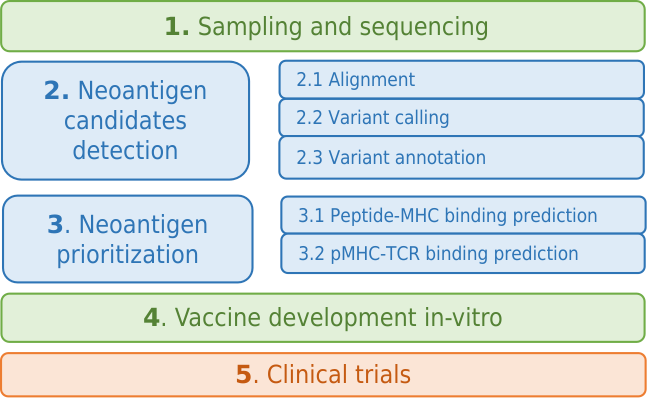
\includegraphics[width=\textwidth]{../img/proposal/vaccine_pipeline}
		\caption{Vaccine process development}
		\label{fig:pipeline_a}
	\end{subfigure}
	\hfill
	\begin{subfigure}[b]{0.55\textwidth}
		\centering
		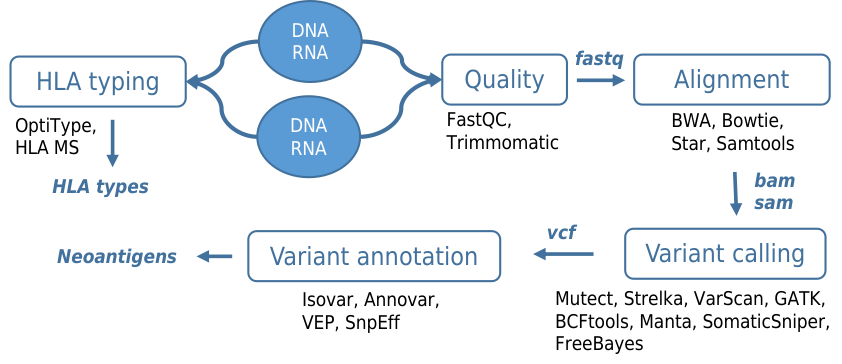
\includegraphics[width=\textwidth]{../img/proposal/neoantigen_detection}
		\caption{Neoantigen detection process}
		\label{fig:pipeline_b}
	\end{subfigure}
	\hfill
	
	\caption{(a) Process to detect neoantigens and develop personalized vaccines. It start by DNA-seq or RNA-seq; then, neoantigen detection is performed followed by neoantigen prioritization; subsequently, a personalized vaccine is develop \textit{in vitro}; and finally, clinical trials are applied. (b) Process for the Detection of neoantigen candidates Initially, DNA/RNA sequencing is conducted on both tumor and normal cells. Subsequently, quality assessment tools are employed, followed by the utilization of alignment tools. The process then proceeds to variant calling to identify variants. Finally, variant annotation tools are applied to generate a list of potential neoantigen candidates. Moreover, MHC typing tools are employed to determine the HLA or MHC types.}
	\label{fig:pipeline}
\end{figure}

\textbf{Neoantigen detection} relies on an initial identification of candidates, which is followed by their subsequent prioritization (stage two and three of Fig. \ref{fig:pipeline_a}). In this project the vaccine development and clinical trials are out of the scope; however they will be included in future works. Detection of neoantigen candidates involves a multi-step process (see Fig. \ref{fig:pipeline_b}). Initially, DNA/RNA sequencing is conducted on both tumor and normal cells. Subsequently, quality assessment tools are employed, followed by the utilization of alignment tools. The process then proceeds to variant calling to identify genetic variants. Finally, variant annotation tools are applied to generate a list of potential neoantigen candidates. In addition to the aforementioned steps, quantitative proteomic tools are utilized for mass spectrometry (MS) data analysis. Moreover, MHC typing tools are employed to determine the Human Leukocyte Antigen (HLA) or Major Histocompatibility Complex (MHC) types.

\textbf{Neoantigen prioritization} is the third stage in cancer vaccines development (Fig. \ref{fig:pipeline_a}). This stage takes candidates neoantigens and then predict their affinity to the Major Histocompatibility Complex (MHC), this problem is know as pMHC binding prediction problem. Then,  this pMHC complex is used to predict the interaction with the T-cell Receptor (TCR). Both problems takes two protein sequences as input, and the goal is to predict their affinity (regression) or binding (classification). In summary, the proteins can be represented as $p = \{ A, ... , Q \}$ and  $q = \{ A, N, K, L, ... ,Q \}$. Then, we need to know the probability of affinity between $p$ and $q$. 

Thus, in this project a method for neoantigen prioritization using Transformer and Transfer Learning is proposed. This method relies on the prediction of pMHC bindings. Moreover, the proposal fine-tuned six pre-trained BERT models adding a block of BiLSTM at the end. Moreover, HLAB dataset \cite{zhang2022hlab} was used for training and testing. Additionally, a layer freezing methodology along with Gradient Accumulation Steps were applied. According to our results, ArgosMHC got promising results outperforming state-of-arts tools like NetMHCpan4.1 \cite{reynisson2020netmhcpan}, MHCFlurry2.0 \cite{o2020mhcflurry}, Anthem \cite{mei2021anthem}, Acme \cite{hu2019acme}, and MixMHCpred2.2 \cite{gfeller2023improved}.

%%%%%%%%%%%%%%%%%%%%%%%%%%%%%%%%%%%%%%%%%%%%%%%%%%%%%%%%%%%%%%%%%%%%%%%%%%%%%%%%%%%%%%%
%%%%%%%%%%%%%%%%%%%%%%%%%%%%%%%%%%%%%%%%%%%%%%%%%%%%%%%%%%%%%%%%%%%%%%%%%%%%%%%%%%%%%%%
\section{Related Works}

Neoantigen detection and prioritization are relevant because of their applications in cancer immunology. As it is a very complex problem, we divided this topic into two categories: (1) the first group together all pipelines developed to detect and prioritize neoantigens; (2) in the second part, we empathized on pMHC binding prediction problem, which is related to neoantigen prioritization.  

\subsection{Pipelines}

A bioinformatic pipeline in the neoantigen context is a software construct that assembles various command line tools. In the problem of neoantigen detection and prioritization, reliance on multiple tools is essential. For instance, we can use tools such as (1) FastQC to ensure sequence quality, (2) BWA handles alignment, (3) Samtools manipulates BAM files, (4) BCFtools is employed for variant calling, (5) Annovar provides variant annotation, and (6) netMHCpan4.1 predicts pMHC binding and pMHC-TCR binding affinity (neoantigen prioritization). However, the use of these diverse tools can introduce compatibility and dependency challenges. To address this issue, developers have created pipeline tools aimed at enhancing the usability of neoantigen detection software. These pipelines effectively manage the integration of these tools, mitigating potential conflicts and dependencies, thereby streamlining the overall neoantigen analysis process.

% definir que es un pipeline (es el framework general), o incluir una figura de un ejemplo de un pipeline.

In Table \ref{tab:review_pipelines}, we present pipelines published since 2018. These pipelines use various types of information as input. For instance, the PGV Pipeline \cite{rubinsteyn2018computational} and PEPPRMINT \cite{zhou2023prioritizing} use DNA-seq, while other tools such as PGNneo \cite{tan2023pgnneo}, NAP-CNB \cite{wert2021predicting}, NaoANT-HILL \cite{coelho2020neoant}, ProGeo-neo \cite{li2020progeo}, ScanNeo \cite{wang2019scanneo}, and Neopepse \cite{kim2018neopepsee} use RNA-seq because these sequences better capture information about mutations and non-coding regions of DNA \cite{tan2023pgnneo}.

To reduce the complexity of pipelines, some proposals have opted to use Variant Calling Format (VCF) as input. These files contain mutation information and are obtained through alignment and mutation calling methods. These tools are: HLA3D \cite{li2022hla3d}, Neoepiscope \cite{wood2020neoepiscope}, pVACtools \cite{hundal2020pvactools}, and NeoPredPipe \cite{schenck2019neopredpipe}. However, the results obtained may be inferior compared to tools that use DNA-seq and RNA-seq.

Additionally, for accurate neoantigen detection, it is necessary to have the sequencing of Major Histocompatibility Complex (MHC) or Human Leukocyte Antigens (HLA) proteins. These proteins are necessary because they are used to predict the binding between potential neoantigens and MHC. These proteins are encoded by highly polymorphic genes, leading to substantial variation in peptide (neoantigen) binding, thereby influencing the set of peptides presented to T-cells \cite{abualrous2021major}. In this context, the  NeoPredPipe \cite{schenck2019neopredpipe}, and Neopepsee \cite{kim2018neopepsee} pipelines request these HLA proteins as input, while others predict this information from DNA-seq. From a usability standpoint, obtaining the HLA types entails unnecessary effort for the user.

As we mentioned before, fusion genes are related to several types of cancer \cite{wood2020neoepiscope,wei2021re,yakushina2018gene,panicker2023exploring,lei2022eml4,zhang2022roles,panagopoulos2023novel}. Thus, there are pipelines which include fusion genes detection methods: Integrate-neo \cite{zhang2017integrate}, neoFusion \cite{wei2019landscape}, pVACfuse \cite{hundal2020pvactools}, NeoepitoPred \cite{chang2017neoepitope}, Epidisco \cite{rubinsteyn2018computational}, TrueNeo \cite{tang2020truneo} and Antigen.garnish \cite{rech2018tumor}. Gene fusions typically yield a higher number of neoantigens per mutation compared to single nucleotide variants (SNVs) and insertions/deletions (Indels). Furthermore, fusion-derived neoantigens exhibit heightened immunogenicity. Notably, neoantigens arising from frameshift fusions or passenger fusions are anticipated to possess the greatest immunogenic potential \cite{wang2021gene}. 

%In general gene fusions can generate more neoantigens per mutation than SNV and Indel. Moreover, Fusion neoantigens seem to be more immunogenic. Specifically, neoantigens derived from frameshift fusions or passenger fusions are predicted to have the highest immunogenicity \cite{wang2021gene}. 


\begin{table}[h]
	\caption{Bioinfomatics pipelines developed for the detection of neoantigens. GN: Gene expression, VA: variant annotation, WEG: whole exome sequencing, WGS: whole genome sequencing.}
	\label{tab:review_pipelines}
	\centering
	\setlength{\tabcolsep}{0.5em} % for the horizontal padding
	{\renewcommand{\arraystretch}{1.1}% for the vertical padding
		{\scriptsize
			\begin{tabular}{p{1.7cm}lp{2.2cm}p{2.2cm}p{7.5cm}}
				\textbf{Name} & \textbf{Year}  & \textbf{Input} & \textbf{Output} & \textbf{Tools} \\ \hline
				PEPPRMINT & 2023  \cite{zhou2023prioritizing} & DNA-seq & Neoantigens & BWA, Mutect, Strelka, ANNOVAR, OptiType, PEPPRMINT, netMHCpan4.1. \\
				PGNneo & 2023	 \cite{tan2023pgnneo}	& VCF, RNA-seq, MS data & Neoantigens & Trimmomatic, BWA, SAMtools, GATK, Picard, OptiType, Annovar, Bedtools, MaxQuant, NetMHCpan4.1, Blastp. \\
				HLA3D & 2022  \cite{li2022hla3d} & VCF, HLA, SMG, HBV & Neoantigens & MHCcluster, SAVES, PROCHECK, CoDockPP, Verify 3D, ERRAT, ClusterW2, 3Dmol, PSRPRED4.0, MHCf lurry. \\
				NextNEOpi & 2022 \cite{dietmar2022nextneopi} & WES/WGS, RNA-seq & Neoantigens & OptiType, pVACseq, NetMHCpan, MHCflurry, NeoFuse, MiXCR. \\
				Seq2Neo & 2022  \cite{Kaixuan2022seq2neo} & WES/WGS, RNA-seq & Neoantigens & Mutect2, STARFusion, ANNOVAR, Agfusion, NetMHCpan, MHCflurry, Pick-Pocket, NetMHCcon, TPMcalculator, NetCTLpan. \\
				%Valid-NEO & 2022 &\cite{terai2022valid} & VCF, HLA & Neoantigens & \\
				NAP-CNB & 2021 \cite{wert2021predicting} & RNA-seq & Neoantigens & Star, Picard, GATK, SplitNCigarsReads, MuTect2, Cufinks, Epi-Seq, pVAC,seq, Neoantimon, MuPeXI, BLOSUM62. \\
				NeoANT-HILL & 2020 \cite{coelho2020neoant} & RNA-seq, VCF  & Neoantigens, GE & GATK, Mutect2, Optitype, NetMHC, NetMHCpan, NetMHCCcons, NetMHCstapan, PickPoket, SMM, SMMPMBEC, MHCflurry, NetMHCIIpan, NN-align, SMM-align, Sturniolo, Kallisto. \\
				Neoepiscope & 2020 \cite{wood2020neoepiscope} & VCF, BAM & Neoantigens & BWA, Bowtie2, Pindel, MuSE, RADIA, SomaticSniper, VarScan2, GATK, HapCUT2. \\
				OpenVax & 2020  \cite{kodysh2020openvax} & DNA-seq, RNA-seq & Neoantigens & GATK 3.7, STAR, MuTect 1.1.7, Mutect 2, Strelka, NetMHCpan, NetMHCCcons, SMM, SMM with a Peptide. \\
				ProGeo-neo & 2020 \cite{li2020progeo} & RNA-seq, VCF & Neoantigens & SRA Toolkit, BWA, GATK, Bcftools, ANNOVAR, Kallisto, OptiType, NetMHCpan4.0. \\
				pVACtools & 2020 \cite{hundal2020pvactools} & VCF & Neoantigens & CWL36, Cromwell37, ADNc38, BWA-MEM25, HaplotypeCaller28, MHCflurry14, MHCnuggets15, NetChop17, INTEGRATE-Neo19. \\
				TruNeo & 2020  \cite{tang2020truneo} & DNA-seq, RNA-seq & Neoantigens & BWA, GATK v3.3, Somatic SNVs, STAR v2.5.3a, RSEM v1.3.0, NetMHCPan 3.0, netChop. \\
				NeoPredPipe & 2019 \cite{schenck2019neopredpipe} & VCF, HLA & Neoantigens, VA & ANNOVAR, POLYSOLVER, netMHCpan, PeptideMatch. \\
				ScanNeo & 2019 \cite{wang2019scanneo} & RNA-seq  & Neoantigens & HISAT2, BEDTools, BWA-MEM, pVAC-Seq, NetMHC, NetMHCpan. \\
				Neopepsee & 2018 \cite{kim2018neopepsee} & RNA-seq, VCF, HLA & Neoantigens, GE & NetCTLpan, Swiss-Prot. \\ 
				PGV Pipeline & 2018 \cite{rubinsteyn2018computational}& DNA-seq & Neoantigens & BWA-MEN, BQSR, MuTect, Strelka, STAR, seq2hla, Vaxrank, Isovar, MHCtools, Varcode, pyEnsembl. \\
			\end{tabular}
		}
	}
\end{table}

\subsection{Neoantigen prioritization}

Neoantigen prioritization depends strongly on the accurate prediction of pMHC bindings. Moreover, the advent of Transformers has ushered in a new era in artificial intelligence, demonstrating significant success across various Natural Language Processing (NLP) tasks \cite{patwardhan2023transformers}. Thus,  several Transformer models have been used for pMHC binding prediction problem. In Table \ref{tab:transformes}, a detailed comparison of Transformers and deep learning methods is presented. For instance, BERTMHC \cite{cheng2021bertmhc} is a pan-specific pMHC-II binding and presentation prediction method that employs a BERT architecture and leverages transfer learning from the Tasks Assessing Protein Embeddings (TAPE) \cite{rao2019evaluating}. The methodology involves stacking an average pooling layer followed by a Fully Connected (FC) layer after the TAPE model. Empirical assessments have shown that BERTMHC outperforms both NetMHCIIpan3.2 and PUFFIN. Additionally, ImmunoBERT \cite{gasser2021interpreting} utilizes transfer learning from TAPE but focuses on pMHC-I prediction. This approach involves stacking a classification token's vector after the TAPE model.
Furthermore, MHCRoBERTa \cite{wang2022mhcroberta} and HLAB \cite{zhang2022hlab} also leverage transfer learning. MHCRoBERTa employs self-supervised training with data from UniProtKB and Swiss-Prot databases, followed by fine-tuning with data from the Immune Epitope Database (IEDB) \cite{vita2019immune}. MHCRoBERTa performs better than NetMHCpan4.0 and MHCflurry2.0 in terms of Spearman Rank Correlation Coefficient (SRCC). In contrast, HLAB leverages transfer learning from ProtBert-BFD \cite{elnaggar2021prottrans} and incorporates a BiLSTM model in cascade. Notably, on the HLA-A*01:01 allele, HLAB demonstrates a slight performance advantage over state-of-the-art methods, including NetMHCpan4.1, with at least a 0.0230 improvement in Area Under the Curve (AUC) and a 0.0560 increase in accuracy. Moreover, in a prior study, we conducted an evaluation of BERT Transformer models using padded sequences for pMHC binding prediction \cite{arceda2023neoantigen}.

Lastly, it's worth noting recent allele-specific research efforts such as TransPHLA \cite{chu2022transformer} and DapNet-HLA \cite{jing2023dapnet}. TransPHLA utilizes peptide self-attention mechanisms and has outperformed existing state-of-the-art methods, including NetMHCpan4.1. %It exhibits efficacy across peptides of varying lengths and MHC alleles, all while demonstrating faster prediction capabilities. 
On the other hand, DapNet-HLA \cite{jing2023dapnet} presents promising results by incorporating an additional dataset (Swiss-Prot) for negative samples and harnessing the strengths of Convolutional Neural Networks (CNNs), SENet for pooling, and Long Short-Term Memory (LSTM) models. %It's important to note that as of now, DapNet-HLA has not been directly compared to existing state-of-the-art methods, making further assessment and comparison necessary. 
Furthermore, there are reviews and benchmarking works \cite{nielsen2020immunoinformatics,mei2020comprehensive,wang2023comprehensive, machaca2023deep,wang2023comprehensive}, which detail the pMHC binding prediction problem. 

In this research, we compared the performance of six Transformer models (TAPE, ProtBert-BFD, ESM2(t6), ESM2(t12), ESM2(t30), and ESM2(t33)) for the task of peptide-MHC class-I binding prediction (pMHC-I). We fine-tuned each model by adding a BiLSTM block in cascade, based on the work of HLAB \cite{zhang2022hlab}. Furthermore, we evaluated the use of Gradient Accumulation Steps and a layer freezing methodology. Our contributions in this study can be summarized as follows: First, a comprehensive assessment and comparison of BERT models, we performed a thorough evaluation of BERT models, utilizing Gradient Accumulation Steps (GAS) and a layer freezing methodology. Following this evaluation, we identified two models, ESM2(t6)-Freeze (ESM2(t6) trained with layer freezing) and TAPE-GAS (TAPE trained with GAS), which achieved the highest scores. The second contribution refers to a comparison of these BERT models with state-of-art tools like NetMHCpan4.1, MHCFlurry2.0, MixMHCpred2.2, Anthem, and ACME. After conducting experiments, ESM2(t6)-Freeze and TAPE-GAS outperformed the other methods, achieving the highest results in terms of Area Under the Curve (AUC), accuracy, recall, f1-score, and Matthews Correlation Coefficient (MCC).


\begin{table}[h]
	\caption{Transformers and deep learning methods with attention mechanism used for pMHC binding prediction.}
	\label{tab:transformes}
	\setlength{\tabcolsep}{0.5em} % for the horizontal padding
	{\renewcommand{\arraystretch}{1.1}% for the vertical padding
		\scriptsize
		%\begin{scriptsize}
		\begin{tabular}{p{1.3cm}p{2.2cm}p{2cm}p{9.5cm}}
			\multicolumn{1}{l}{\textbf{Year}}                                   & \textbf{Name}             & \textbf{Input}            & \textbf{Model}     \\  \hline
			
			2023\cite{hashemi2023improved}&	ESM-GAT  &	One-hot & BERT with transfer learning from ESM1b and ESM2 fine-tuned with a Graph Attention Network (GAT) at the end. It outperformed NetMHCpan4.1.	\\
			
			
			2023\cite{kalemati2023capsnet}&	CapsNet-MHC&	BLOSUM62 & Capsule Neural Network, it outperformed state-of-art tools for small peptides of 8 to 11-mer.	\\
			
			2023\cite{ye2023stmhcpan}&	STMHCpan  &	One-hot & A Star-Transformer model, it use usefull for anylenght peptides and could extended for predicting T-cell responses.	\\
			
			2023\cite{jing2023dapnet}&	DapNet-HLA&	Fused word embedding & Combined the advantages of CNN, SENet (for pooling), and LSTM with attention.	\\
			
			2022\cite{zhang2022hlab}&	HLAB&	One-hot & BERT from ProtBert pre-trained model followed by a BiLSTM with attention mechanism.	\\
			
			2022\cite{wang2022mhcroberta}          & MHC RoBERTa            & One-hot &  RoBERTa  pre-trained and followed by 12 multi-head SA and a FC layers, it outperformed NetMHCPan 3.0.                                                                                          \\
			2022\cite{chu2022transformer}          & TransPHLA             & One-hot         & It used SA mechanism based on four blocks, it slightly outperformed NetMHCpan4.1 and is faster making predictions.\\
			
			2021\cite{chen2021jointly}  & CapTransformer            & One-hot   &  Transformer with cross attention pooling to capture local and global information.  \\
			
			2021\cite{gasser2021interpreting}  & ImmunoBERT            & One-hot                     & BERT from TAPE pre-trained followed by a linear layer. Authors claimed that N-terminal and C-terminals are highly relevant after analysis with SHAP and LIME.   \\
			
			2021\cite{cheng2021bertmhc}             & BERTMHC              & One-hot                    & BERT from TAPE pre-trained followed by a linear layer. It outperformed NetMHCIIpan3.2 and PUFFIN.   \\
			
			% CNN and RNN with attention
			2021\cite{ye2021mathla}         & MATHLA             & BLOSUM                      & 
			It integrates BiLSTM with multi-head attention. It achieved an AUC score of 0.964, compared to 0.945, 0.925 and 0.905 for netMHCpan 4.0, MHCflurry and ACME respectively  \\
			
			2021\cite{liu2021deepseqpanii}                    & DeepSeqPanII                            & BLOSUM62 and one-hot& It has two LSTM layers, an attention block and three FC layers. It got better results than NetMHCIIpan 3.2 on 26 of 54 alleles.       \\
			
			2021\cite{yang2021deepnetbim}  & DeepNetBim               & BLOSUM50            & It uses separate CNNs for pMHC binding and immunogenetic with a attention module. It got 0.015 MAE for binding and 94.7 of accuracy for immunogenic.      \\
			
			2021\cite{jin2021deep}         & DeepAttentionPan        & BLOSUM62            & CNN with an attention mechanism. It is allele-specific and got slightly better results than ACME for allele level.     \\
			
			2021\cite{chen2021ranking}  & SpConvM            &  One-hot, BLOSUM, and Deep                     &  1D layer of CNN, an attention  layer and a FC layer. Moreover, they employed global kernels to enhance their results, along with a combination of onehot, BLOSUM, and Deep.  \\
			
			2020 \cite{venkatesh2020mhcattnnet}         & MHCAttNet        & One-hot            & CNN followed by an attention layer to generate a heat map over the amino acids.     \\
			
			2019\cite{hu2019acme}          & ACME                     & BLOSUM50     & CNN with  attention, it extract interpretable patterns  about pMHC binding. Moreover, it got SRCC of 0.569, AUC of 0.9 for HLA-A and 0.88 for HLA-B.  \\    
			
			
			2019\cite{wu2019deephlapan}                      & DeepHLApan                              & One-hot             & Allele-specific model with three layers of Bidirectional GRU (BiGRU) with an attention layer. It got acc $> 0.9$ on 43 HLA alleles.                                               
		\end{tabular}
		%	\end{scriptsize}
}
\end{table}




\section{Proposal}

The proposal is divided into two contributions: first, the development of a method using Transformers and Transfer learning for neoantigen prioritization; second, the development of a pipeline which integrates bioinformatics tools including ArgosMHC.

\subsection{ArgosMHC}

The project encompass an assessment and comparison of six Transformer models: TAPE \cite{rao2019evaluating}, ProtBert-BFD \cite{elnaggar2021prottrans} and ESM2 \cite{lin2023evolutionary} (ESM2(t6), ESM2(t12), ESM2(t30), ESM2(t33)). These models were trained with large protein sequences datasets like Pfam \cite{el2019pfam}, and BFD and UniRef50  \cite{suzek2015uniref}. We fine-tuned these models for the task of pMHC binding prediction problem. Moreover, this study looked for the benefits of using a layer freezing methodology.  In Table \ref{tab:pretrained}, we present the characteristics of each model.


\subsubsection{Pre-trained transformers}

\textbf{Tasks Assessing Protein Embeddings} (TAPE) \cite{rao2019evaluating} is the first attempt to evaluate semi-supervised learning on protein sequences. TAPE has twelve layers of 512 units with eight attention heads, achieving 92 million parameters. The authors applied semi-supervised training with Pfam dataset \cite{el2019pfam}, which has thirty million protein domains. Furthermore, the Pfam dataset is derived from UniProt Knowledge (UniProtKB) \cite{uniprot2018uniprot}; in particular, Pfam used sequences that belong to Reference Proteomes \cite{finn2016pfam} instead of using the entire UniProtKB dataset. Consequently, Pfam has almost half of the protein sequences that other datasets based on UniProtKB. 



\textbf{ProtBert-BFD} is part of a family of ProtTrans \cite{elnaggar2021prottrans} models. The authors evaluated several deep learning architectures with BFD, UniRef50, and UniRef100 datasets, each with 2122, 45, and 216 million sequences. For instance, BFD is considered the most extensive collection of protein sequences; it merged UniProt \cite{uniprot2019uniprot} and proteins from multiple meta-genomics sequencing projects. Meanwhile, UniRef \cite{suzek2015uniref} provides a clustered set of protein sequences from UniProtKB. Notably, the larger dataset, BFD, is more noisy; it has sequence mistakes \cite{elnaggar2021prottrans}. Some models proposed are ProtBert-BFD, ProtT5-XL and ProtT5-XXL, which have 420 million, 3 billion, and 11 billion parameters, respectively. ProtBert-BFD were trained with BFD; meanwhile, ProtT5 models were initially trained with BFD and then with UniRef50, which improved performance by 2.8\% and 1.4\% for ProtT5-XL and ProtT5-XXL respectively. Nevertheless, ProtT5-XL outperformed both ProtBert-BFD and the biggest model ProtT5-XXL. The authors claimed that the number of samples increased performance but didn't observe similarity consistent with model size. They suggested that larger models see fewer samples in the same computing power, so larger models need larger datasets. For that reason, we have opted for ProtBert as it is smaller than ProtT5-XL, and we believe it is better suited to the current dataset size.



\textbf{ESM-2} \cite{lin2023evolutionary} is a family of transformer models that scales from 8 million to 15 billion parameters. The model is based on BERT \cite{devlin2018bert}, outperforming its previous version ESM-1b \cite{rives2021biological} by removing dropout in hidden and attention layers. Furthermore, the authors suggested that absolute positional encoding methods don't extrapolate well; consequently, they used Rotary Position Embedding (RoPE). Significantly, with the use of RoPE, the training cost is slightly increased; meanwhile, it improves model quality for small models \cite{lin2023evolutionary}. Moreover, the authors used the non-redundant  UniRef50 \cite{suzek2015uniref} dataset from UniProt, with 60 million protein sequences. 


\begin{table}[]%
	\centering
	\caption{Significant differences between TAPE, ProtBert-DFB, and ESM2 models. ESM2 has four models of different sizes. HS: Hidden size, AH: Attention heads}
	\label{tab:pretrained}%
	\scriptsize
	\begin{tabular}{llrrrrr}
		\hline
		\textbf{Model}   & \textbf{Dataset} & \textbf{Samples} & \textbf{Layers} & \textbf{HS} & \textbf{AH} & \textbf{Params.} \\
		\hline
		TAPE             & Pfam             & 30M                   & 12              & 768                  & 12                       & 92M                 \\
		ProtBert-BFD     & BFD              & 2122M                 & 30              & 1024                 & 16                       & 420M                \\
		ESM2(t6)  & Uniref50         & 60M                   & 6               & 320                  & 20                       & 8M                  \\
		ESM2(t12)  & Uniref50         & 60M                   & 12              & 480                  & 20                       & 35M                 \\
		ESM2(t30) & Uniref50         & 60M                   & 30              & 640                  & 20                       & 150M                \\
		ESM2(t33)  & Uniref50         & 60M                   & 33              & 1280                 & 20                       & 650M               \\
		\hline
	\end{tabular}
	
\end{table}
 
 
 \subsubsection{Fine tuning}\label{sec:fine-tuned}
 
 For fine-tuning, we stacked in cascade a BiLSTM at the end of the pre-trained model. The BiLSTM is based on HLAB \cite{zhang2022hlab} and has two layers with 768 units.  In Fig. \ref{fig:finetune}, we present the whole model for pMHC-I binding prediction. 
 
 
 \begin{figure}[h]
 	\centering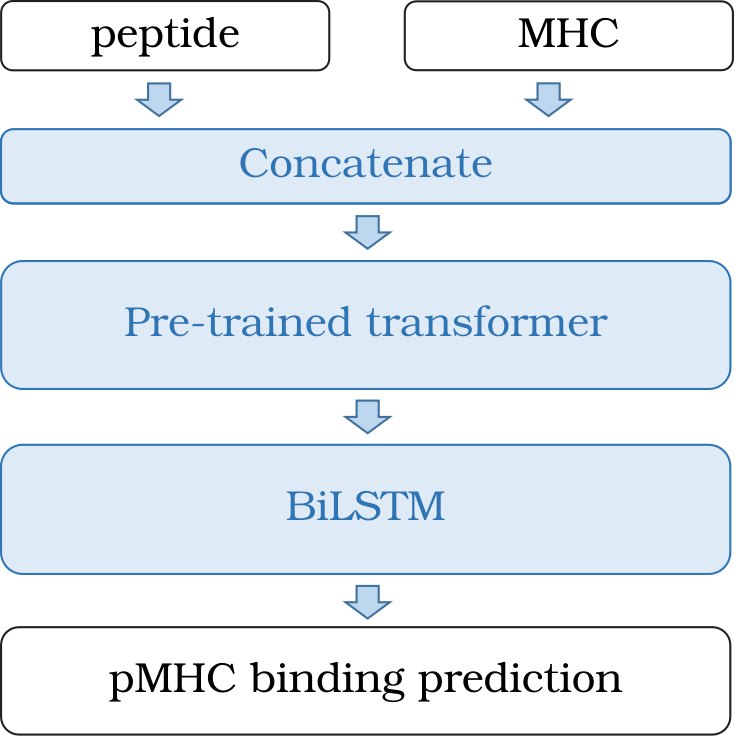
\includegraphics[width=0.2\textwidth]{../img/proposal/pipeline}
 	\caption{The proposed architecture for pMHC-I binding prediction using a pre-trained transformer model and a BiLSTM block stacked in cascade.}
 	\label{fig:finetune}
 \end{figure}
 
 Moreover, it is well-established that when fine-tuning large transformer models, the final layers exhibit more significant changes, while the initial layers, closer to the input, undergo relatively minor modifications \cite{merchant2020happens,lee2019would,kovaleva2019revealing}. Consequently, we compared the results of freezing the pre-trained model and only updating the BiLSTM parameters versus updating the whole model parameters. 
 
 Furthermore, large transformer models run out of GPU memory. Therefore, inspired by similar works training transformer models \cite{anil2021large,zhang2023adam,huang2023measuring}, we evaluated the results of applying gradient accumulation steps during training.
 
 Finally, we used the following hyperparameters: learning rate of 5e-5, weight decay of 0.0001, momentum of 0.9, warmup steps of 1000 with linear decay, ADAM optimizer ($\beta_1 = 0.9, \beta_2=0.999$), and early stopping. These values were used by BERTMHC \cite{cheng2021bertmhc} after a grid search.

\subsection{NeoArgosTools}
\section{Experiments and Results}

\subsection{Dataset}
We used peptide sequences from the Anthem dataset \cite{mei2021anthem}. It consists of 539019, 179673, and 172580 samples for training, validation, and testing, respectively. In more detail, in Fig. S1, we present the distribution of samples by k-mers; 9-mers comprise the majority of samples in the database.

\subsection{Binary classifier and metrics}
The pMHC binding prediction problem is a regression problem. Nonetheless, based on the dataset employed in this study, it could also be approached as a binary classification problem by selecting an appropriate threshold. Moreover, the machine learning metrics used in this work are: Accuracy (Acc.), Precision (Precis.), Recall, F1-score (F1-sc), and Area Under the Curve (AUC).

\subsection{Vanishing gradients}
At the beginning of the experiments, the bigger models suffered from the vanishing gradients problem. Thus, according to best practices to fine-tune the BERT model \cite{mosbach2020stability}, we evaluated lower learning rates, increased the warmup steps in the learning scheduler, and used ADAM with bias correction. So, we evaluated three configurations: (c3) $lr=2e-5$ and 20k warnup steps, (c4) $lr=1e-5$ and 100k warnup steps, and (c5) $lr=2e-6$ and 200k warnup steps. In Fig. \ref{fig:loss}, the loss comparison during training is plotted. In this case, we see that configuration three is good for the smaller model ESM2(t6); however, the same configuration didn't work for the bigger model ESM2(t33). Moreover, in Fig. \ref{fig:t6_c3_gradients} the layer one's gradients of ESM2(t6) show a normal behavior; meanwhile, in Fig. \ref{fig:t33_c3_gradients}, we can see how gradients of the bigger model tend to zero. Thus, configuration four and five were evaluated; sadly, configuration four also went to vanishing gradients. Meanwhile, configuration five overcame that problem according to Fig. \ref{fig:t33_c5_gradients}. For that reason, Configuration Five was applied to the following experiments.

\begin{figure}[h]
	\centering
	
	\begin{subfigure}[b]{0.45\textwidth}
		\centering
		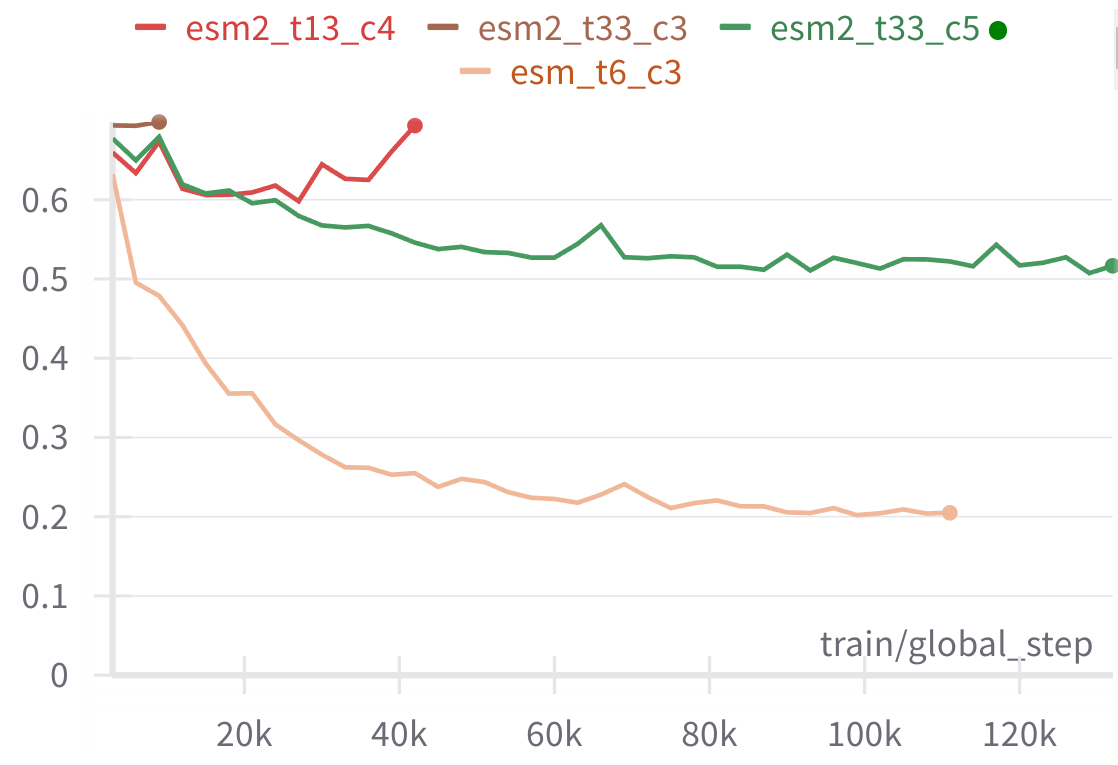
\includegraphics[width=\textwidth]{../img/results/loss2}
		\caption{Loss}
		\label{fig:loss}
	\end{subfigure}
	\hfill
	\begin{subfigure}[b]{0.45\textwidth}
		\centering
		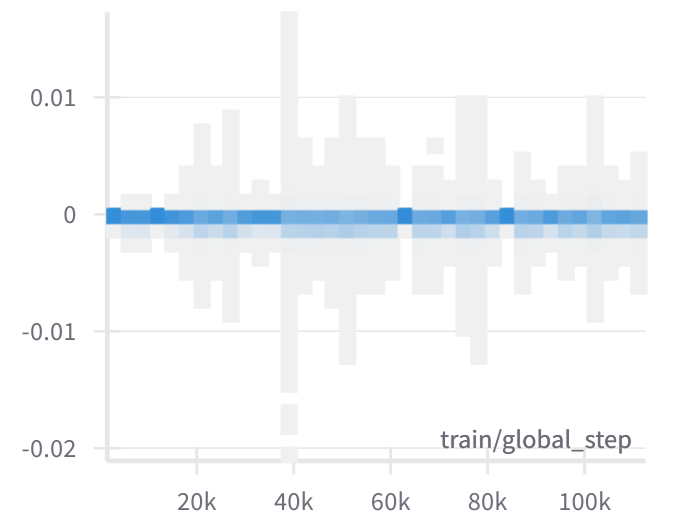
\includegraphics[width=\textwidth]{../img/results/t6_c3_gradients}
		\caption{ESM2(t6) Configuration 3.}
		\label{fig:t6_c3_gradients}
	\end{subfigure}
	\hfill
	\begin{subfigure}[b]{0.45\textwidth}
		\centering
		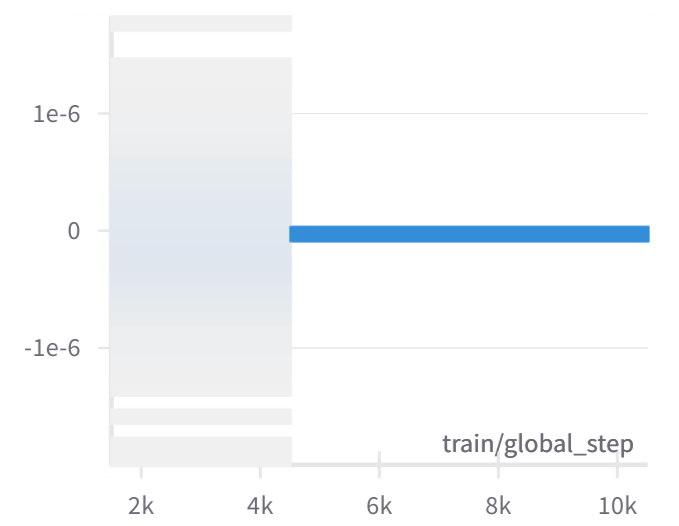
\includegraphics[width=\textwidth]{../img/results/t33_c3_gradients}
		\caption{ESM2(t33) Configuration 3.}
		\label{fig:t33_c3_gradients}
	\end{subfigure}
	\hfill
	\begin{subfigure}[b]{0.45\textwidth}
		\centering
		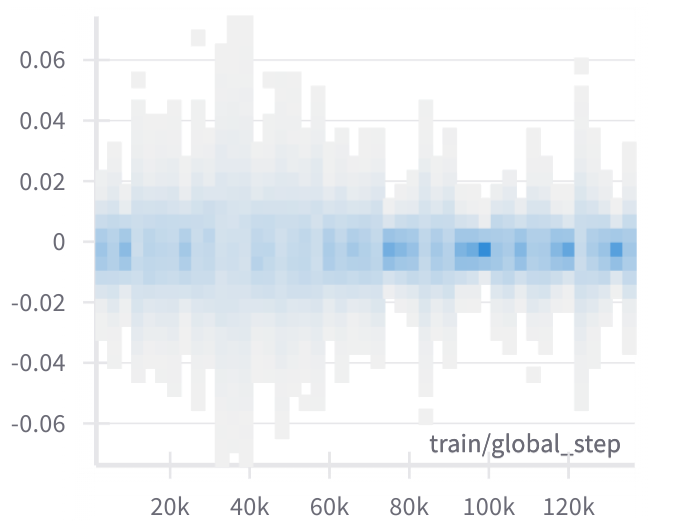
\includegraphics[width=\textwidth]{../img/results/t33_c5_gradients}
		\caption{ESM2(t33) Configuration 5.}
		\label{fig:t33_c5_gradients}
	\end{subfigure}
	
	%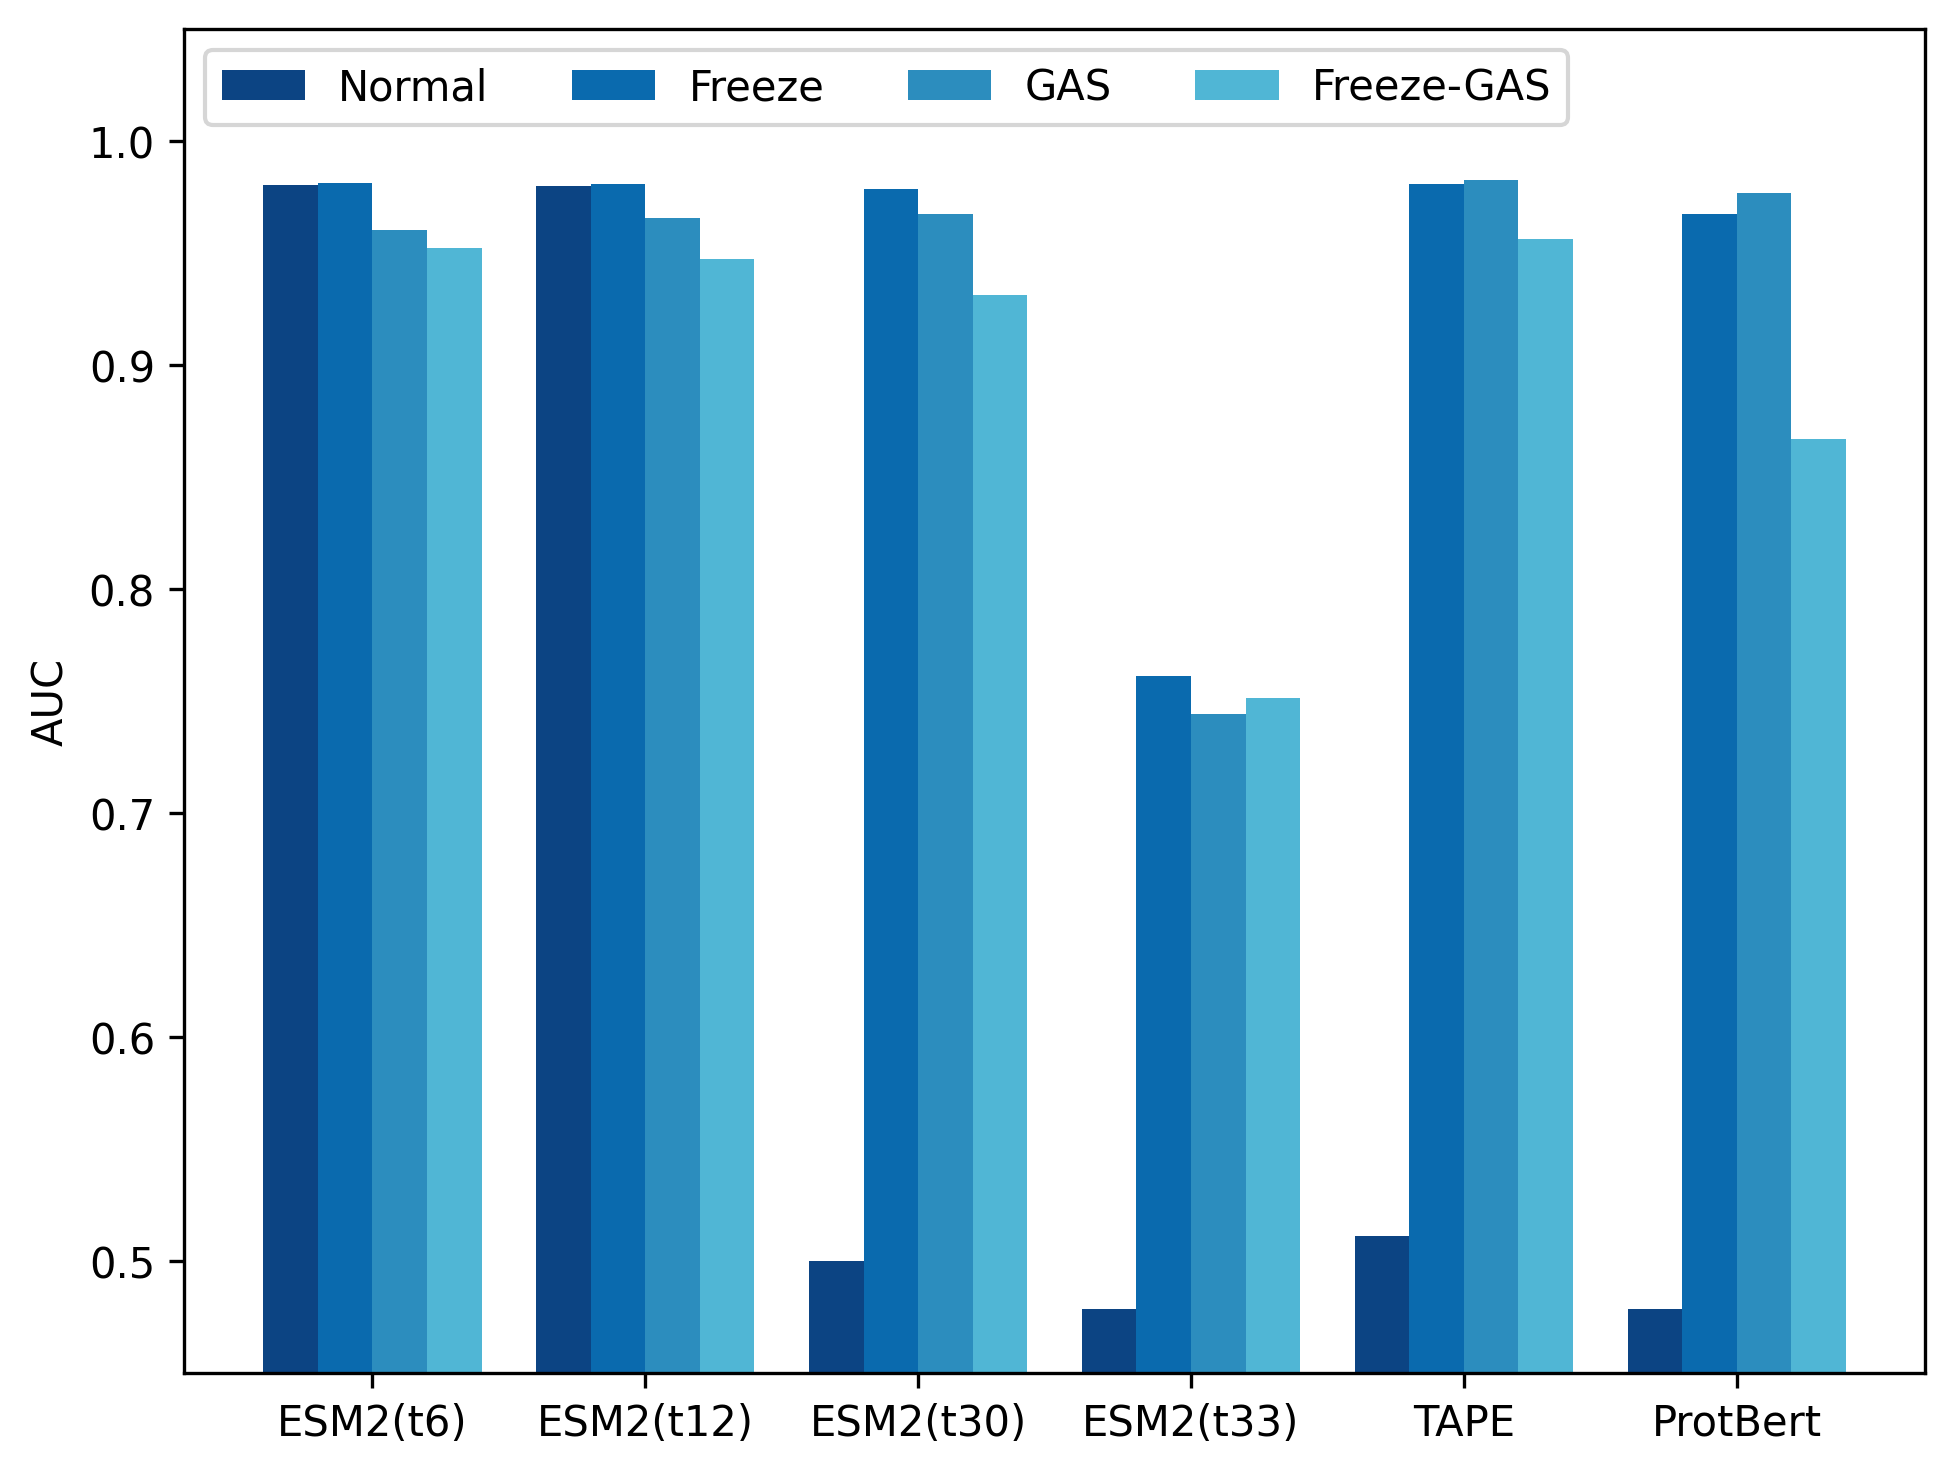
\includegraphics[width=0.42\textwidth]{../img/results/metrics_comparion_by_model}	
	
	\caption{(a) Loss during training of three configurations varying the learning rate and warmup steps. (b) First layer's gradients of ESM2(t6) using third configuration. (c) First layer's gradients of ESM2(t33) using the fourth configuration. (d) First layer's gradients of ESM2(t33) using the fifth configuration.}
	\label{fig:training}
\end{figure}


\subsection{The layer freezing methodology and GAS}

For the layer freezing methodology, we froze all the Transformer's parameters and just trained the BiLSTM block. Using this method speeds up the training and still achieves good performance, as discussed in prior works \cite{merchant2020happens,lee2019would,kovaleva2019revealing}. The performance comparison is presented in Table \ref{tab:comparison_3_epochs}; the suffix 'GAS' signifies the integration of Gradient Accumulation Steps (GAS), while the suffix 'Freeze' is indicative of our application of the layer freezing methodology to the models.

\begin{figure}[h]
	\centering
	
	
	
	\begin{subfigure}[b]{0.45\textwidth}
		\centering
		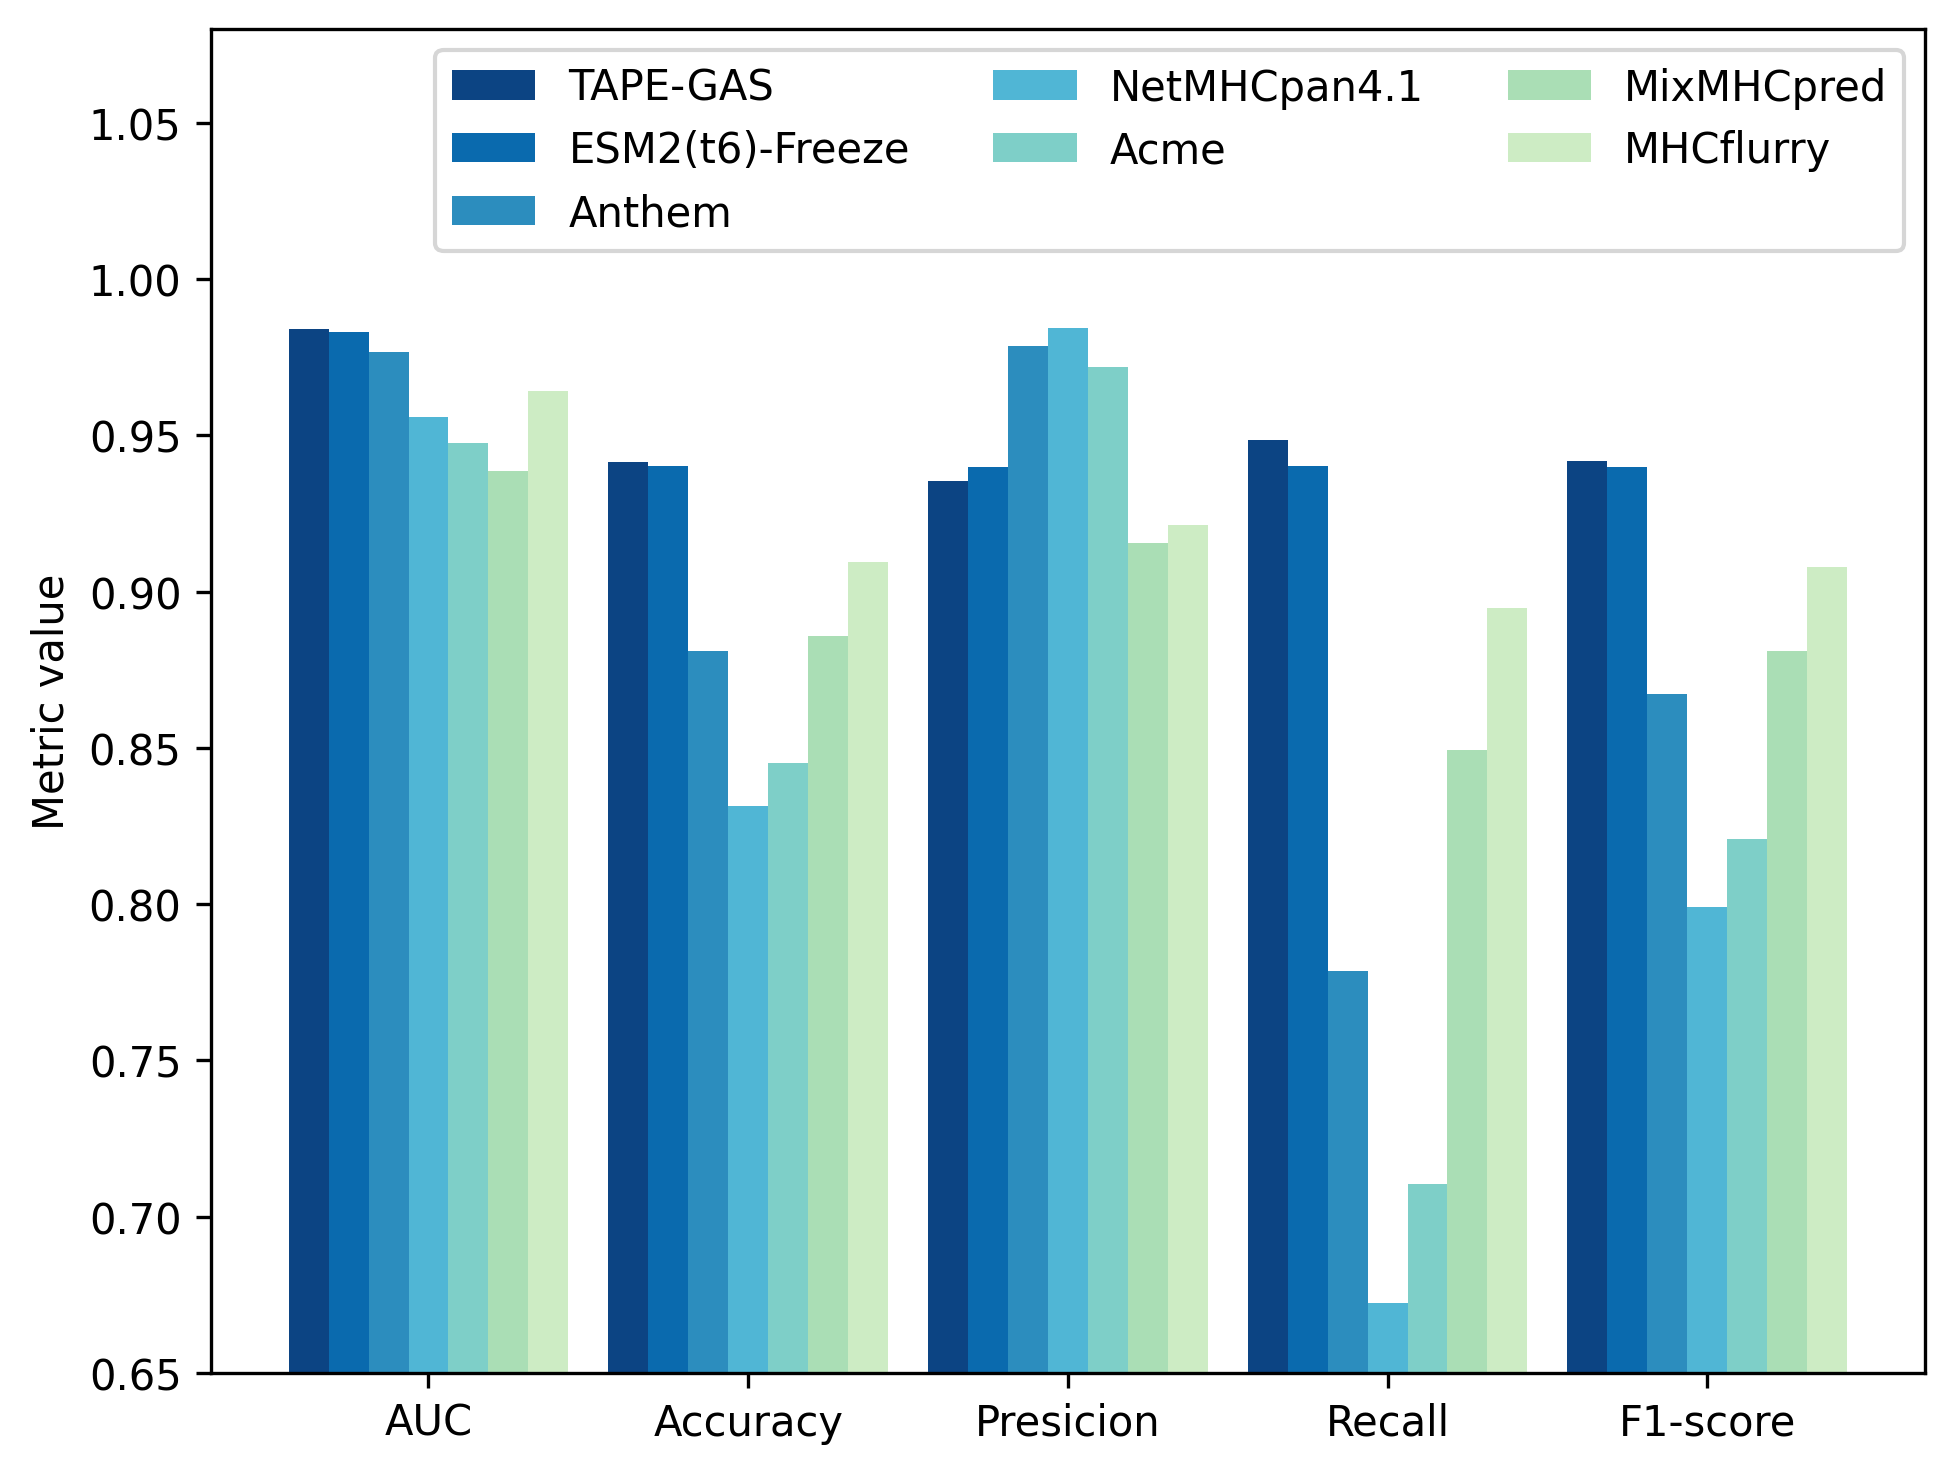
\includegraphics[width=\textwidth]{../img/results/metrics_comparison}
		\caption{Thirty epochs}
		\label{fig:comparison_final}
	\end{subfigure}
	\hfill
	\begin{subfigure}[b]{0.45\textwidth}
		\centering
		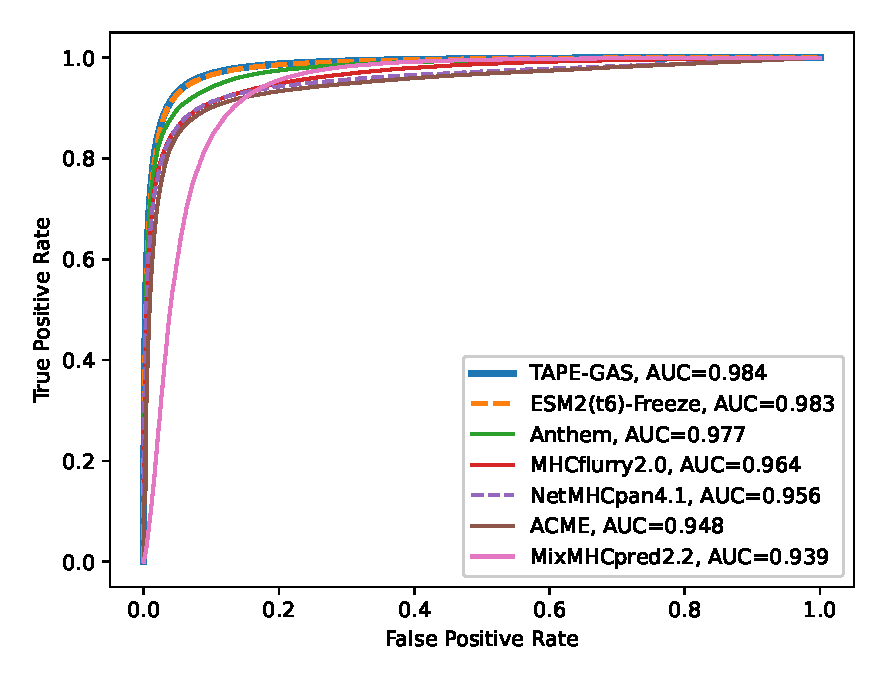
\includegraphics[width=\textwidth]{../img/results/ROC_comparison}
		\caption{ROC curves}
		\label{fig:ROC_comparison_final}
	\end{subfigure}
	
	%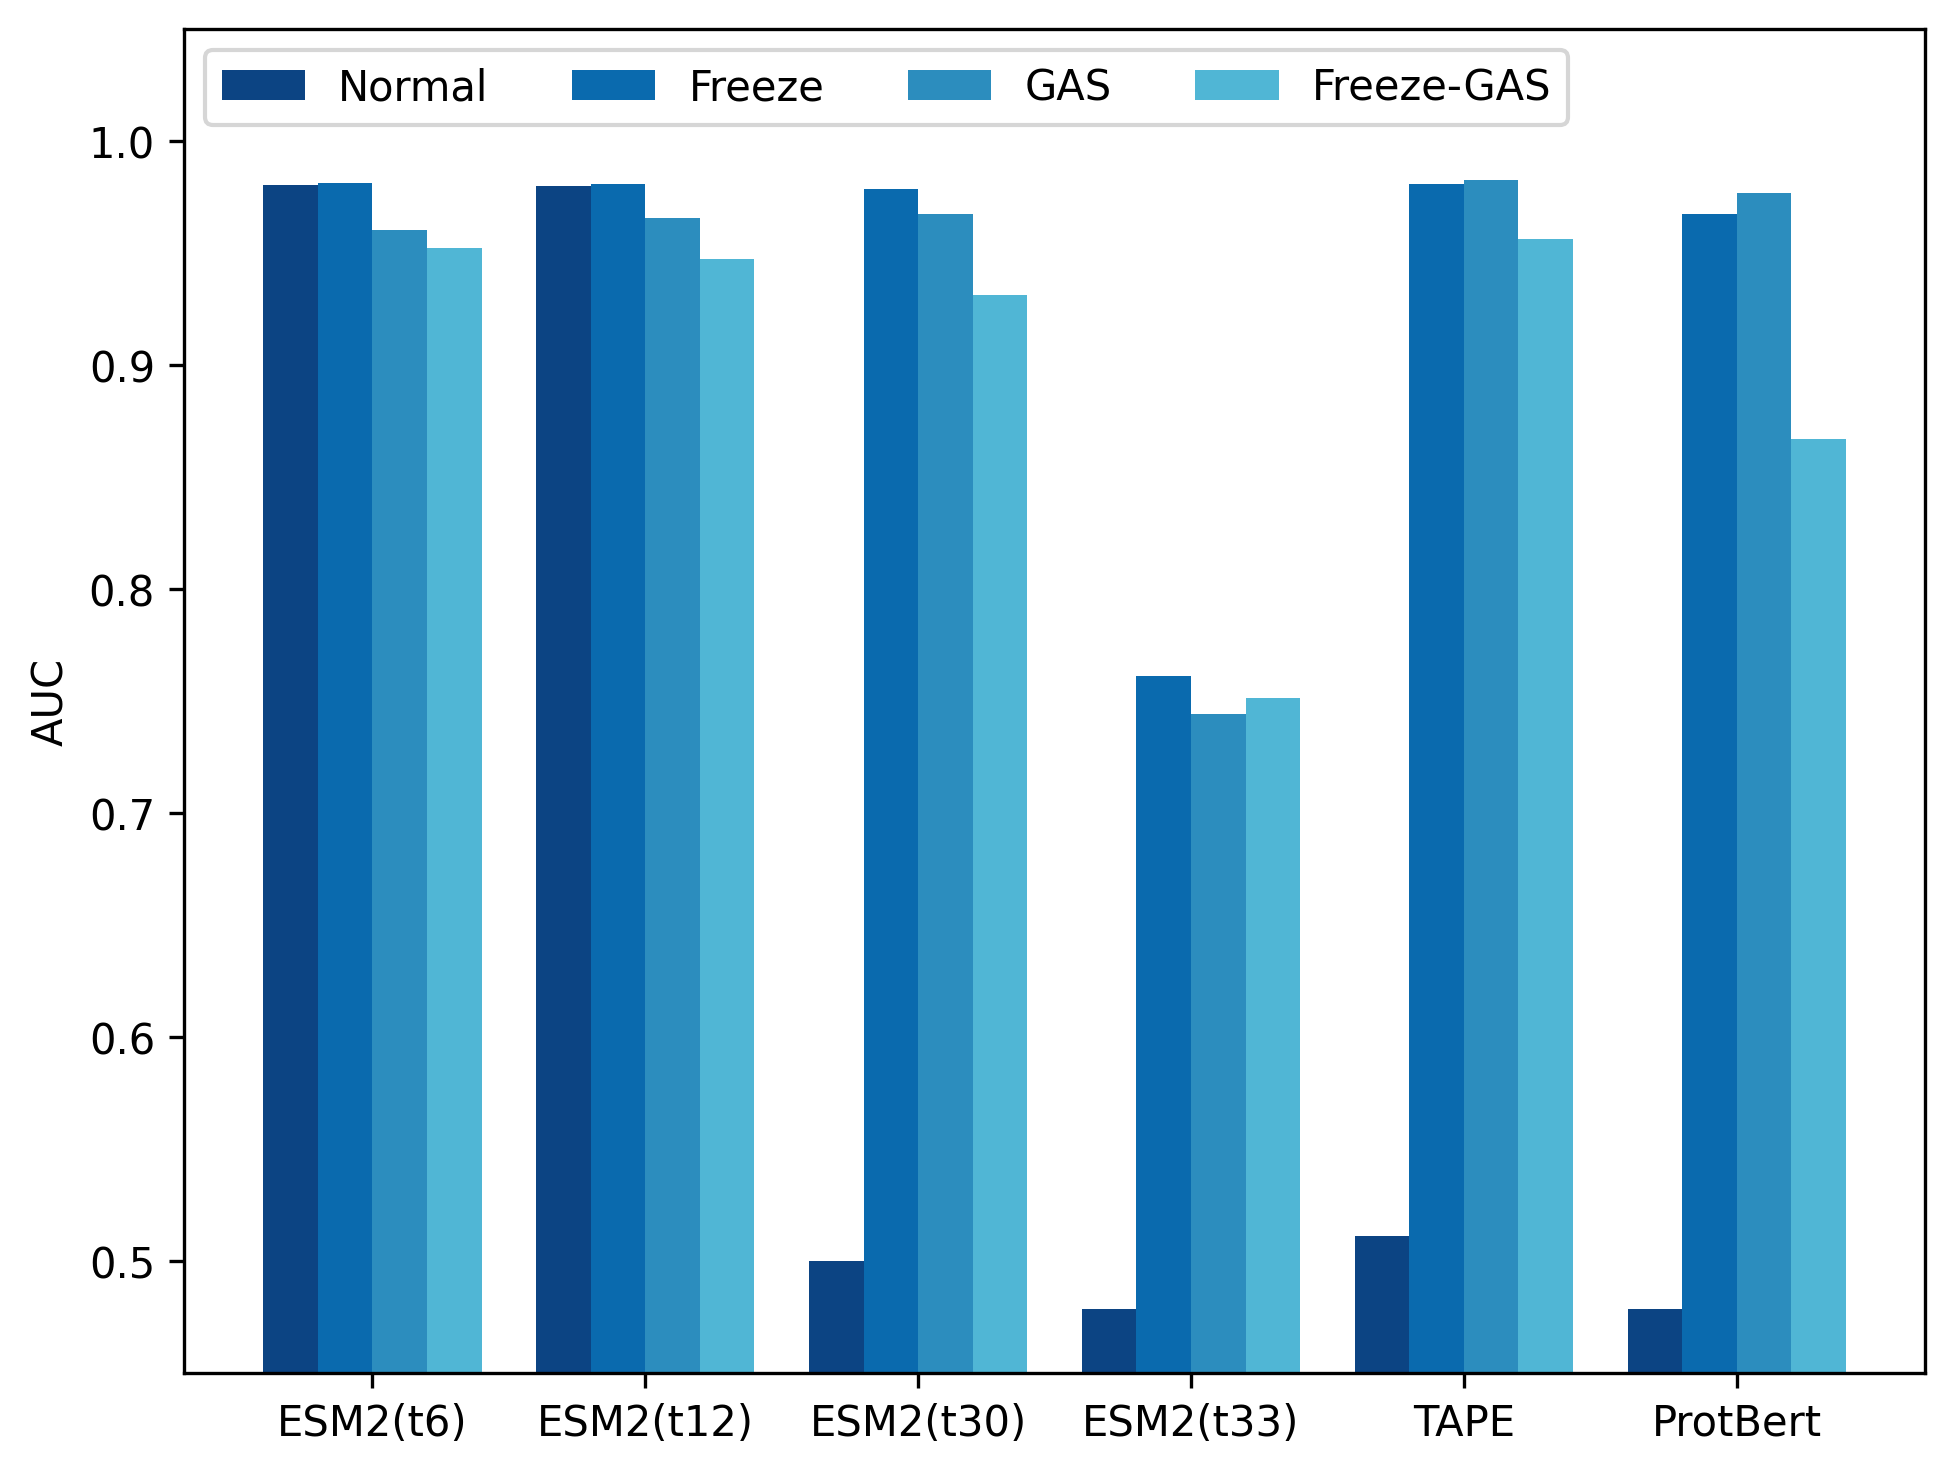
\includegraphics[width=0.42\textwidth]{../img/results/metrics_comparion_by_model}	
	
	\caption{(a) The AUC values for TAPE-GAS and ESM2(t6) trained for 30 epochs, in comparison to state-of-the-art methods. (b) ROC curves for TAPE-GAS and ESM2(t6) trained for 30 epochs, in comparison to state-of-the-art methods.}
	\label{fig:comparison}
\end{figure}





\begin{table}[h]
	\centering
	\caption{Performance evaluation of Transformer models with Gradient Accumulation Steps (GAS) and the layer freezing methodology trained for three epochs. Moreover, the suffix 'Normal' stands for classic training. The inclusion of the suffix 'GAS' in each model signifies the integration of Gradient Accumulation Steps, while the suffix 'Freeze' is indicative of our application of the layer freezing methodology to the models.}
	\label{tab:comparison_3_epochs}
	
	\scriptsize
	\begin{tabular}{llllll} \hline
		\textbf{Model}       & \textbf{Acc.} & \textbf{Precis.} & \textbf{Recall} & \textbf{F1-sc.} & \textbf{AUC}   % & \textbf{MCC}    
		\\ \hline
		ESM2(t6)-Normal             & 0.9344            & \textbf{0.9334}    & 0.9354          & 0.9344            & 0.9805          %& 0.8689          
		\\
		ESM2(t6)-Freeze      & \textbf{0.9351}   & 0.9253             & \textbf{0.9464} & \textbf{0.9357}   & \textbf{0.9812} %& \textbf{0.8704} 
		\\
		ESM2(t6)-GAS         & 0.8986            & 0.8966             & 0.9007          & 0.8986            & 0.9602          %& 0.7973          
		\\
		ESM2(t6)-Freeze-GAS  & 0.8869            & 0.8913             & 0.8806          & 0.8860            & 0.9520          %& 0.7738          
		\\ \hline
		
		
		ESM2(t12)-Normal            & 0.9327            & 0.9243             & 0.9422          & 0.9332            & 0.9799          %& 0.8655          
		\\
		ESM2(t12)-Freeze     & \textbf{0.9344}   & \textbf{0.9251}    & \textbf{0.9451} & \textbf{0.9350}   & \textbf{0.9808} %& \textbf{0.8690} 
		\\
		ESM2(t12)-GAS        & 0.9010            & 0.9279             & 0.8692          & 0.8976            & 0.9655          %& 0.8037          
		\\
		ESM2(t12)-Freeze-GAS & 0.8805            & 0.8556             & 0.9149          & 0.8843            & 0.9475          %& 0.7629          
		\\ \hline
		
		
		ESM2(t30)-Normal             & 0.8923                 & 0.8956                  & 0.9076               & 0.9034                 & 0.9467               %&                & -               %& -               
		\\
		ESM2(t30)-Freeze     & \textbf{0.9303}   & \textbf{0.9185}    & \textbf{0.9440} & \textbf{0.9311}   & \textbf{0.9786} %& \textbf{0.8609} 
		\\
		ESM2(t30)-GAS        & 0.9090            & 0.9167             & 0.8993          & 0.9079            & 0.9675          %& 0.8181          
		\\
		ESM2(t30)-Freeze-GAS & 0.8565            & 0.8156             & 0.9206          & 0.8649            & 0.9312          %& 0.7191          
		\\ \hline
		
		
		ESM2(t33)-Normal            & 0.6797                 & 0.7122                  & 0.8076               & 0.7220                 & 0.7458               %& -               
		\\
		ESM2(t33)-Freeze     & \textbf{0.6818}   & \textbf{0.7139}    & 0.6044          & 0.6546            & \textbf{0.7613} %& 0.3677          
		\\
		ESM2(t33)-GAS        & 0.6767            & 0.6312             & 0.8467          & 0.7233            & 0.7442         % & \textbf{0.3763} 
		\\
		ESM2(t33)-Freeze-GAS & 0.6738            & 0.6254             & \textbf{0.8633} & \textbf{0.7254}   & 0.7514          %& 0.3763          
		\\ \hline
		
		
		TAPE-Normal             & 0.8986                 & 0.8245                  & 0.9045               & 0.8845                 & 0.9267                           
		\\
		TAPE-Freeze          & 0.9342            & 0.9276             & 0.9415          & 0.9345            & 0.9809          %& 0.8684          
		\\
		TAPE-GAS             & \textbf{0.9371}   & \textbf{0.9290}    & \textbf{0.9463} & \textbf{0.9376}   & \textbf{0.9826} %& \textbf{0.8744} 
		\\
		TAPE-Freeze-GAS      & 0.8914            & 0.8851             & 0.8989          & 0.8920            & 0.9564          %& 0.7828          
		\\ \hline
		
		
		ProtBert-Normal          & 0.7456                 & 0.7045                  & 0.7205               & 0.7599                 & 0.7178               %&
		\\
		ProtBert-Freeze      & 0.9083            & 0.9176             & 0.8968          & 0.9071            & 0.9673          %& 0.8168          
		\\
		ProtBert-GAS         & \textbf{0.9138}   & \textbf{0.9569}    & 0.8662          & \textbf{0.9093}   & \textbf{0.9767} %& \textbf{0.8313} 
		\\
		ProtBert-Freeze-GAS  & 0.7864            & 0.7333             & \textbf{0.8988} & 0.8076            & 0.8669          %& 0.5881         
		\\ \hline
	\end{tabular}
\end{table}



For a more detailed comparison, we extended the training epochs of the best-performing models from Table \ref{tab:comparison_3_epochs}, including ESM2(T6) and TAPE, to 30 epochs with early stopping. It is worth noting that ProtBert-BFD was excluded from the analysis due to its poor performance. As indicated in Table \ref{tab:comparison}, the ESM2 models yield their best results when the layer freezing methodology is applied. In contrast, for TAPE, the best results are achieved when using GAS without freezing. Notably, TAPE-GAS and ESM2(t6)-Freeze produced the most favorable outcomes, with TAPE-GAS slightly outperforming ESM2(t6)-Freeze in this regard.




\begin{table}[h]
	\centering
	\caption{Performance evaluation of Transformer models with GAS and the layer freezing methodology, trained for thirty (30) epochs. Moreover, the suffix 'Normal' stands for classic training. The inclusion of the suffix 'GAS' in each model signifies the integration of GAS, while the suffix 'Freeze' is indicative of our application of the layer freezing methodology to the models.}
	\label{tab:comparison}
	\scriptsize
	\begin{tabular}{llllll} \hline
		\textbf{}            & \textbf{Acc.} & \textbf{Precis.} & \textbf{Recall} & \textbf{F1-sc.} & \textbf{AUC}      \\ \hline
		ESM2(t6)-Normal             & 0.9390            & 0.9333             & \textbf{0.9453} & 0.9392            & 0.9797                    \\
		
		ESM2(t6)-Freeze      & \textbf{0.9401}   & \textbf{0.9398}    & 0.9402          & \textbf{0.9400}   & \textbf{0.9830}          \\
		ESM2(t6)-GAS         & 0.9366            & 0.9322             & 0.9413          & 0.9368            & 0.9818                           \\
		ESM2(t6)-Freeze-GAS  & 0.9354            & 0.9326             & 0.9383          & 0.9355            & 0.9813                             \\ \hline
		
		TAPE-Normal        & 0.9086                 & 0.9399                  & 0.9281               & 0.9145                 & 0.9648                                 \\
		TAPE-Freeze          & 0.9395            & \textbf{0.9404}    & 0.9382          & 0.9393            & 0.9815                           \\
		TAPE-GAS             & \textbf{0.9415}   & 0.9352             & \textbf{0.9484} & \textbf{0.9418}   & \textbf{0.9841}            \\
		TAPE-Freeze-GAS      & 0.9359            & 0.9297             & 0.9428          & 0.9362            & 0.9820                    \\ \hline    
	\end{tabular}
\end{table}


\subsection{Comparison with state-of-art methods}
Additionally, we compare the best models: ESM2(t6)-Freeze and TAPE-GAS trained for 30 epochs (see Table \ref{tab:comparison}) with state-of-art methods. We covered NetMHCpan4.1 \cite{reynisson2020netmhcpan}, and MHCFlurry2.0 \cite{o2020mhcflurry} because are well-know baselines methods; and three latest tools such as Anthem \cite{mei2021anthem},  Acme \cite{hu2019acme} and MixMHCpred2.2  \cite{gfeller2023improved}. 
During our evaluation of these tools on the test dataset, we encountered specific considerations for ACME. To ensure a fair assessment, we excluded the following alleles from the evaluation for ACME: HLA-C01:02, HLA-C02:02, HLA-C03:03, HLA-C03:04, HLA-C04:01, HLA-C05:01, HLA-C06:02, HLA-C07:01, HLA-C07:02, HLA-C07:04, HLA-C08:02, HLA-C12:03, HLA-C14:02, HLA-C15:02, HLA-C16:01, HLA-C17:01, HLA-A02:50, HLA-A24:06, HLA-A24:13, HLA-A32:15, HLA-B45:06, and HLA-B83:01. This exclusion was necessary as ACME was unable to predict peptide-MHC binding for these particular alleles,

It's worth noting that the choice of threshold for predicting pMHC binding can vary depending on the specific tool and k-mer used. This variability makes the AUC an ideal metric for comparing methods, as it provides a robust evaluation that isn't sensitive to threshold differences. For that reason, in  Figure \ref{fig:comparison_final} and \ref{fig:ROC_comparison_final}, we present the AUC and ROC curve respectively of TAPE-GAS, ESM2(t6)-Freeze, NetMHCpan4.1, and MHCFlurry2.0, Anthem,  Acme, and MixMHCpred2.2. According to these plots, TAPE-GAS, ESM2(t6)-Freeze got the highest AUC value.

Furthermore, when assessing binary classification performance metrics, we standardized the threshold for TAPE-GAS and ESM2(t6) at 0.5. We maintained a threshold of 0.5 for NetMHCpan4.1, in accordance with its recommended setting, while for ACME, we adhered to a threshold of 0.42, as advised in its documentation. In the case of Anthem, the tool provided binary binding predictions directly. However, for MixMHCpred2.2 and MHCfurry, we determined the optimal threshold values from the test dataset, resulting in 2.7308 and 0.09439, respectively. In Table \ref{tab:final_comparison}, we present a comprehensive comparison between TAPE-GAS and ESM2(t6)-Freeze (trained for 30 epochs), and state-of-the-art methods. The results clearly demonstrate that TAPE-GAS and ESM2(t6)-Freeze consistently outperform the existing state-of-the-art tools across all these metrics: AUC, Accuracy, Recall, F1-score, and MCC. 


\begin{table}[h]
	\centering
	\caption{Performance evaluation of Transformer models TAPE-GAS and ESM2(t6)-Freeze, trained for 30 epochs, against Anthem, NetMHCpan4.1, ACME, MixMHCpred2.2, and MhcFlurry2.0.}
	\label{tab:final_comparison}
	\scriptsize
	\begin{tabular}{lllllll} \hline
		& \textbf{Acc.} & \textbf{Precis.} & \textbf{Recall} & \textbf{F1-sc} & \textbf{AUC}    & \textbf{MCC}    \\ \hline
		TAPE-GAS        & \textbf{0.9415}   & 0.9352             & \textbf{0.9484} & \textbf{0.9418}   & \textbf{0.9841} & \textbf{0.8831} \\
		ESM2(t6)-Freeze & \textbf{0.9401}   & 0.9398             & \textbf{0.9402} & \textbf{0.9400}   & \textbf{0.9830} & \textbf{0.8802} \\
		
		Anthem          & 0.8811            & \textbf{0.9786}    & 0.7787          & 0.8673            & 0.9768          & 0.7785          \\
		NetMHCpan4.1    & 0.8312            & \textbf{0.9844}    & 0.6724          & 0.7991            & 0.9557          & 0.6982          \\
		
		ACME            & 0.8452            & 0.9717             & 0.7105          & 0.8208            & 0.9476          & 0.7165          \\
		MixMHCpred2.2   & 0.8857            & 0.9155             & 0.8493          & 0.8811            & 0.9386          & 0.7733          \\
		MhcFlurry2.0    & 0.9093            & 0.9211             & 0.8948          & 0.9078            & 0.9642          & 0.8189 \\ \hline        
	\end{tabular}
\end{table}


Finally, we show the AUC distribution for TAPE-GAS and ESM2(t6)-Freeze, both trained for 30 epochs, along with Anthem, NetMHCpan4.1, ACME, MixMHCpred2.2, and MHCflurry2.0. In this case, we evaluated each distribution by k-mer (Fig. \ref{fig:auc_distribution}). In all k-mer, TAPE-GAS and ESM2(t6)-Freeze present the highest score. Furthermore, it's worth noting that the compact ESM2(t6)-Freeze model delivers superior results for longer peptides with lengths of 11, 12, 13, and 14.


\begin{figure*}[h]
	\centering
	%\begin{subfigure}[b]{0.3\textwidth}
	%	\centering
	%	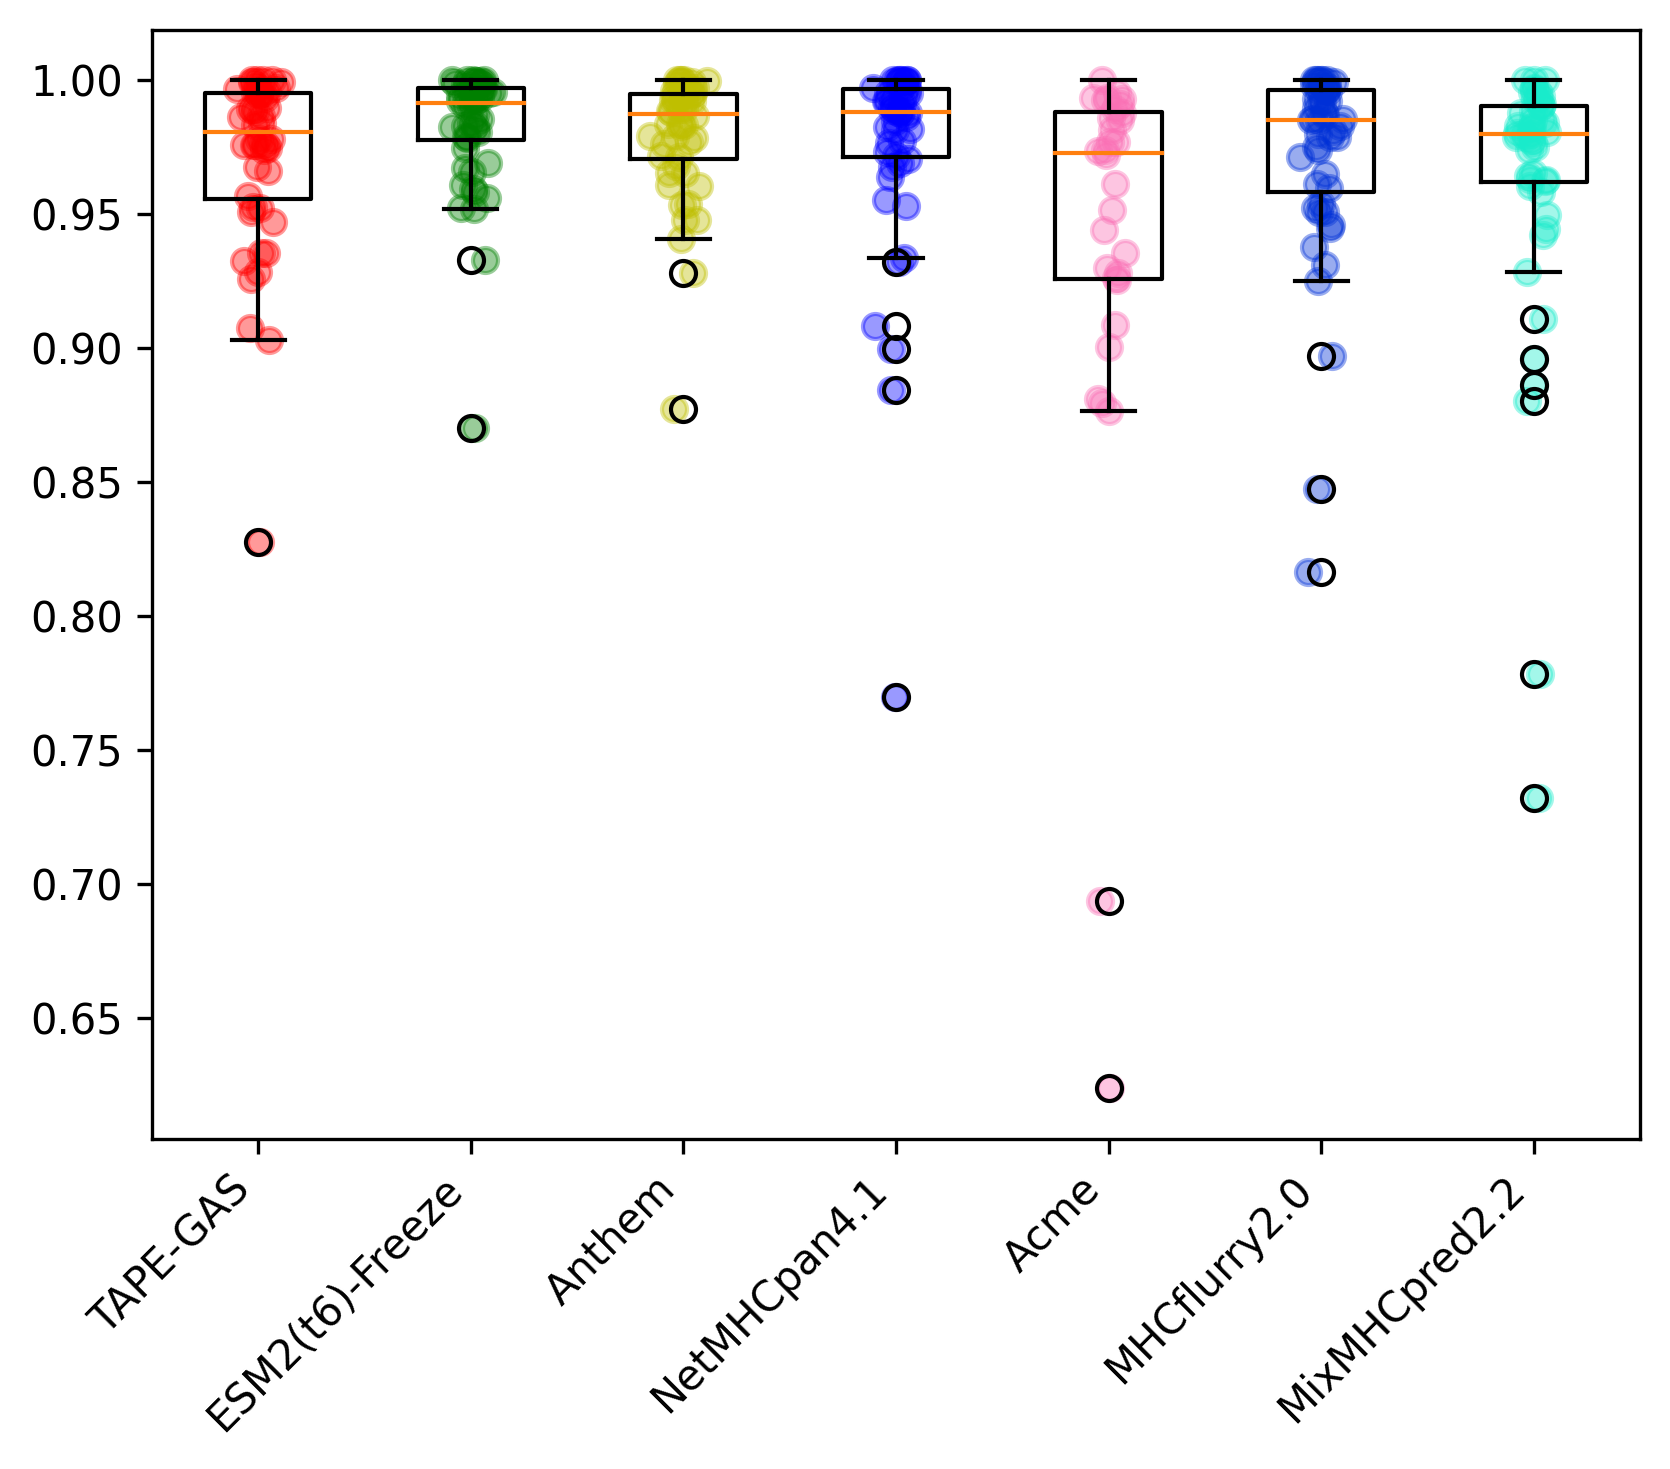
\includegraphics[width=\textwidth]{img/results/auc_distribution_8-mer.eps}
	%	\caption{8-mer}
	%	\label{fig:comparison_8}
	%\end{subfigure}
	%\hfill
	\begin{subfigure}[b]{0.3\textwidth}
		\centering
		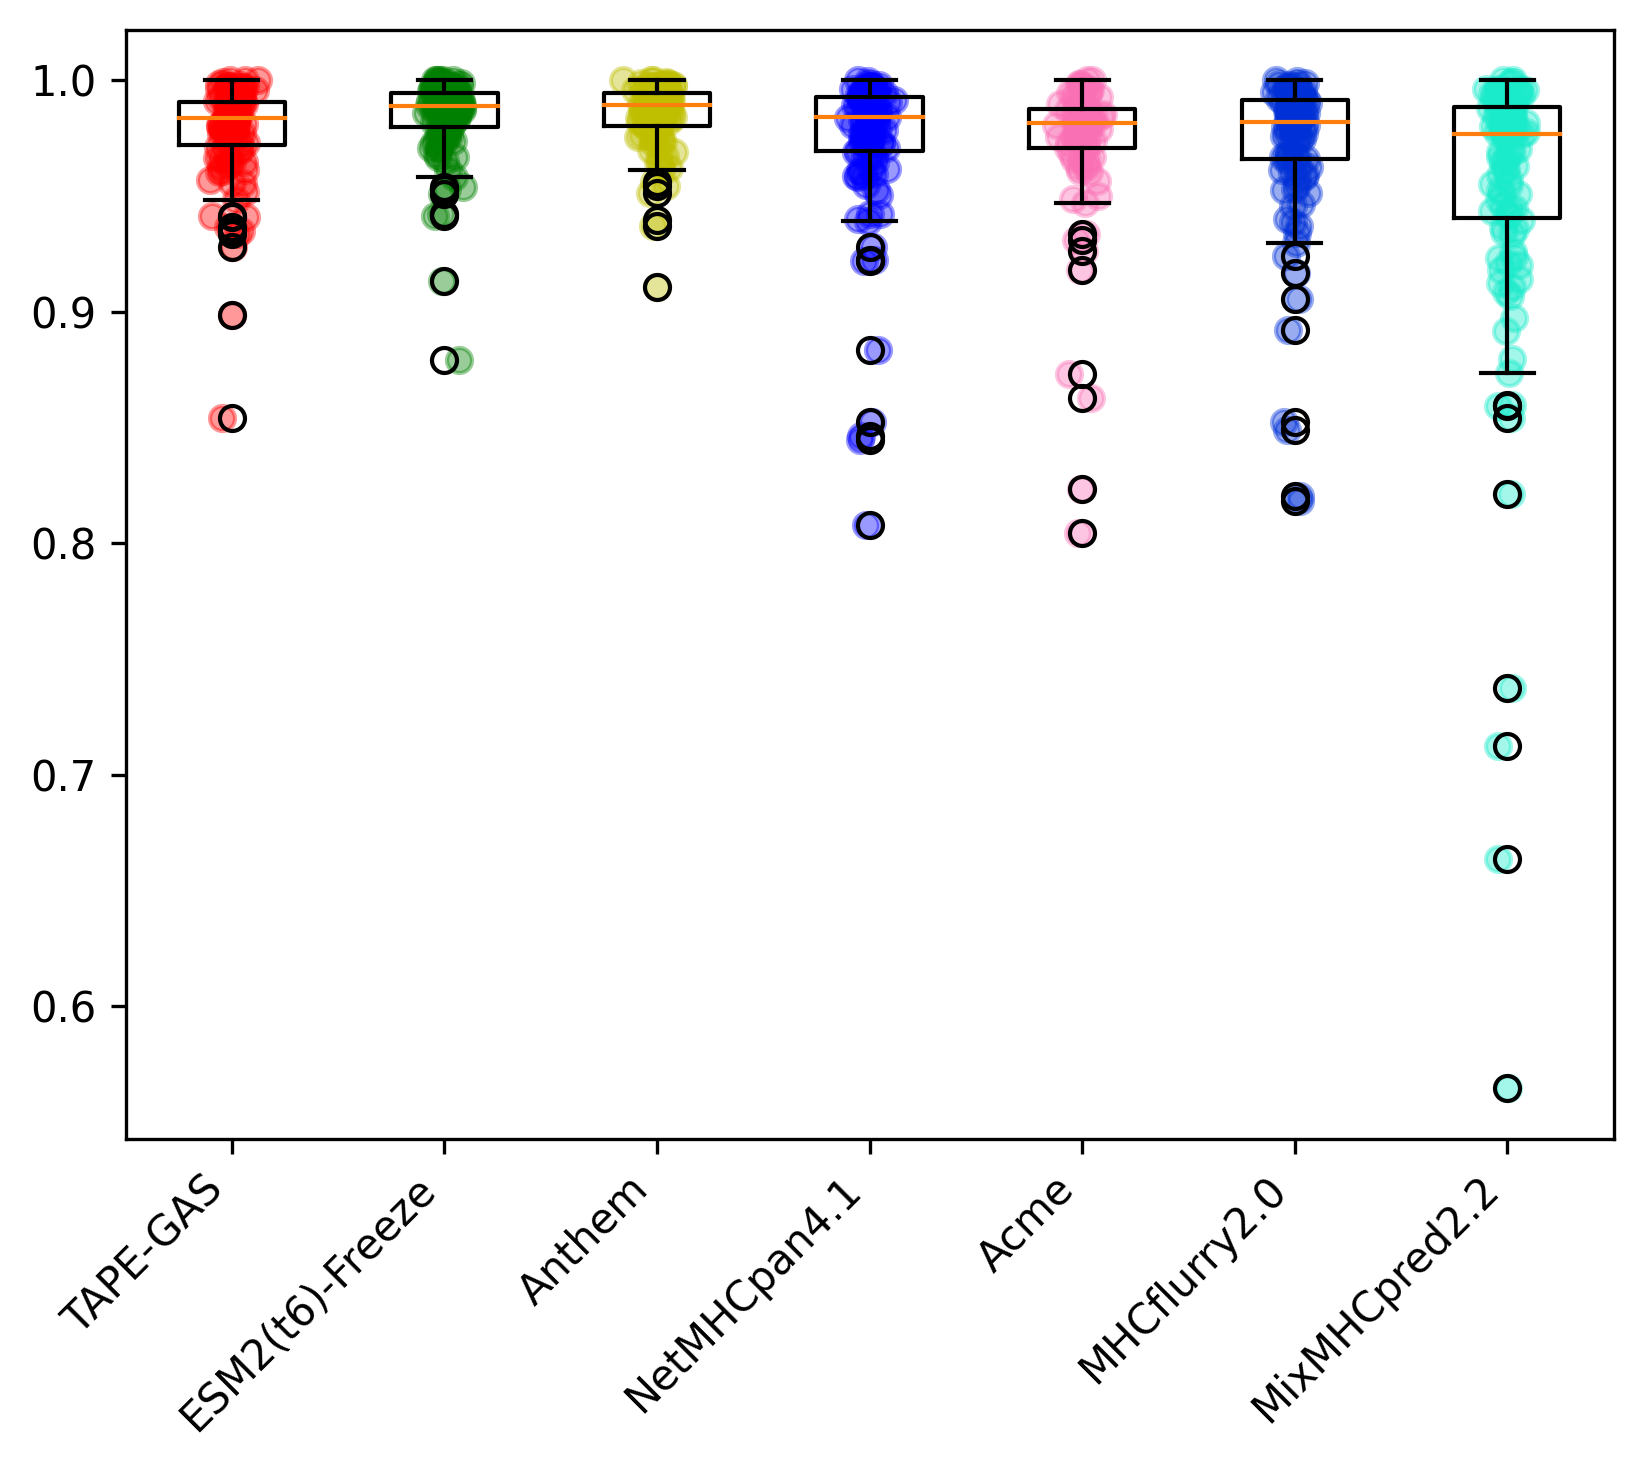
\includegraphics[width=\textwidth]{../img/results/auc_distribution_9-mer}
		\caption{9-mer}
		\label{fig:comparison_9}
	\end{subfigure}
	\hfill
	\begin{subfigure}[b]{0.3\textwidth}
		\centering
		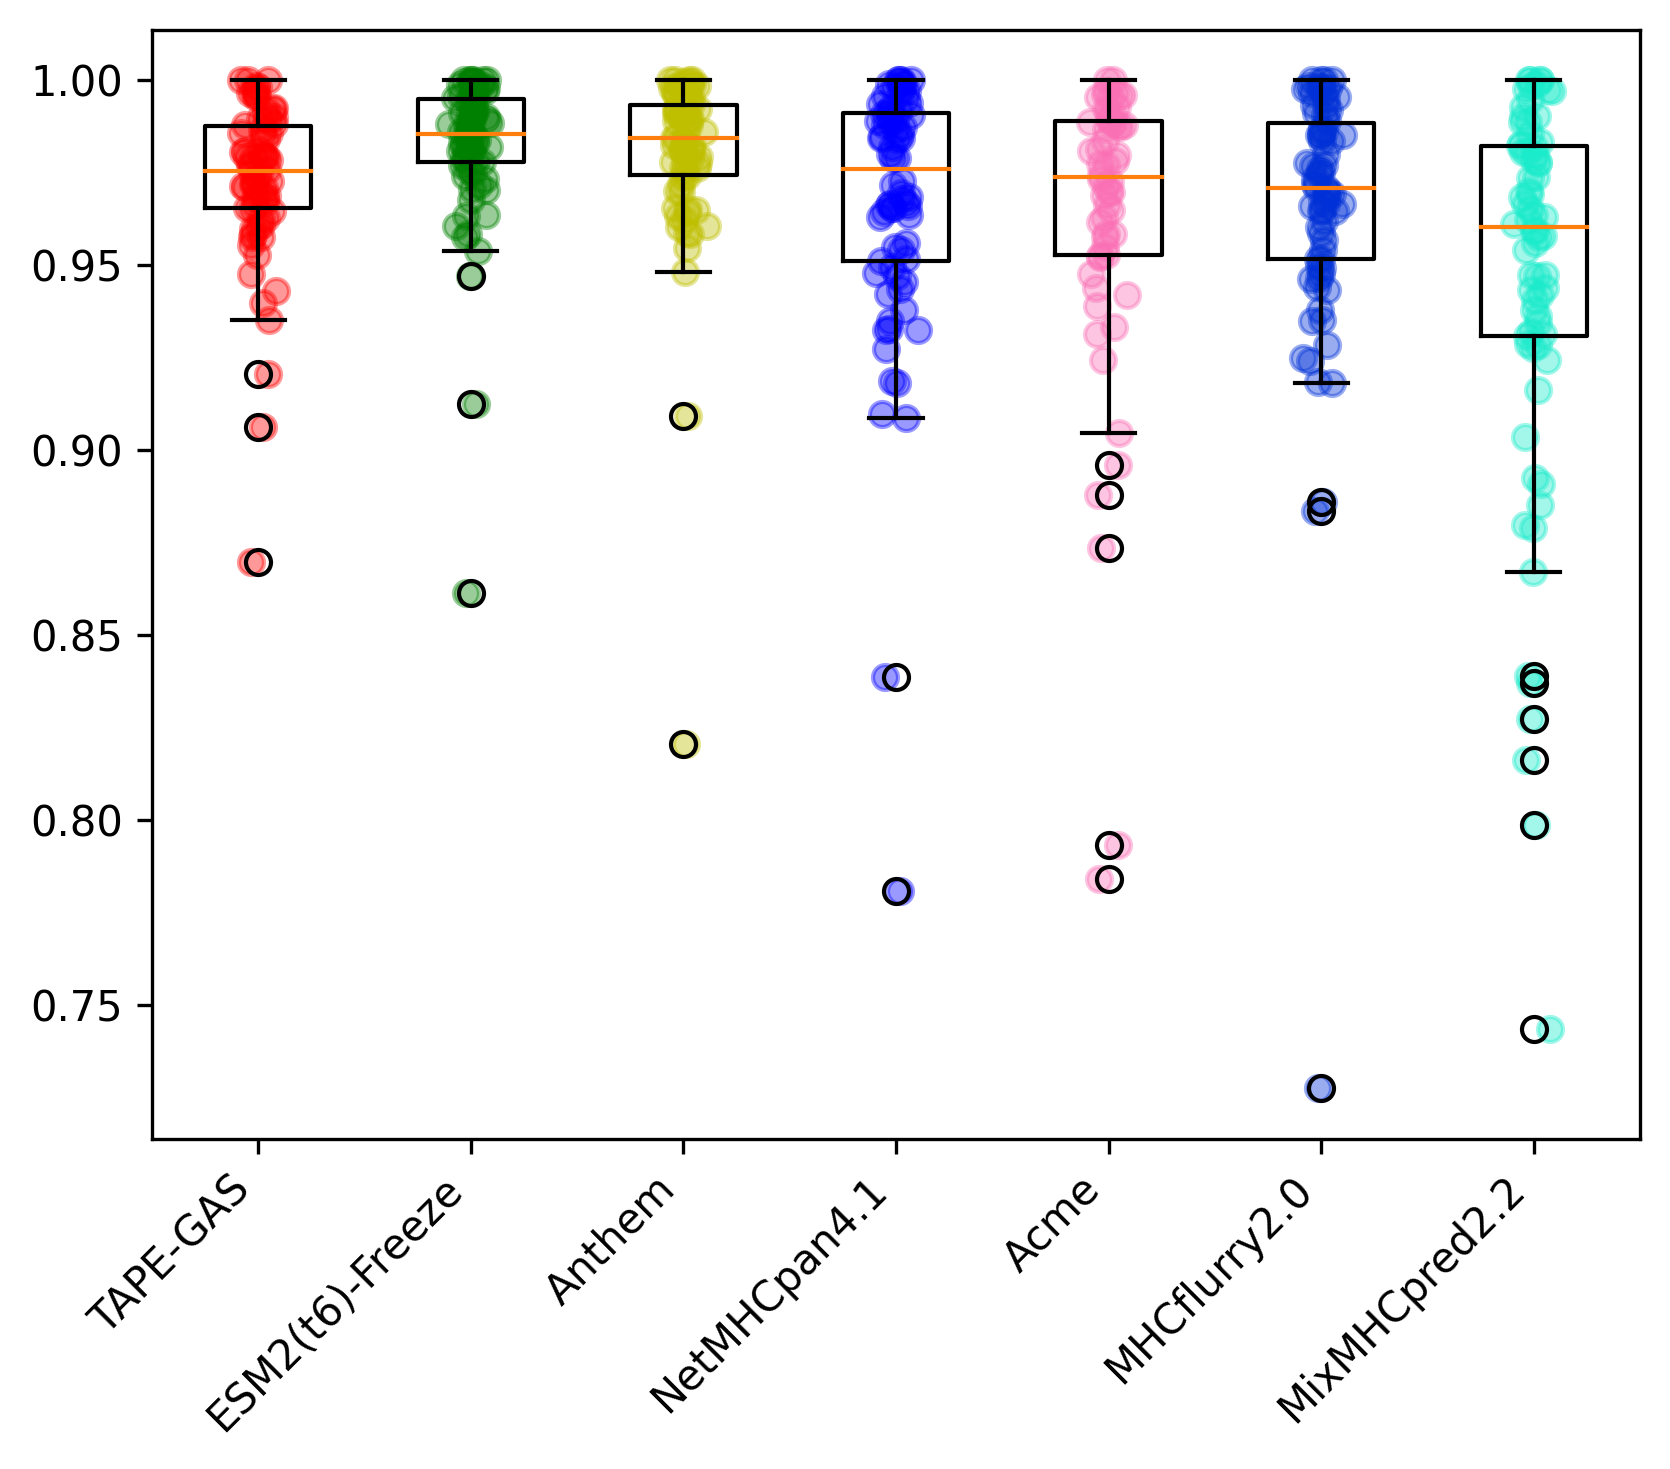
\includegraphics[width=\textwidth]{../img/results/auc_distribution_10-mer}
		\caption{10-mer}
		\label{fig:comparison_10}
	\end{subfigure}
	\hfill
	\begin{subfigure}[b]{0.3\textwidth}
		\centering
		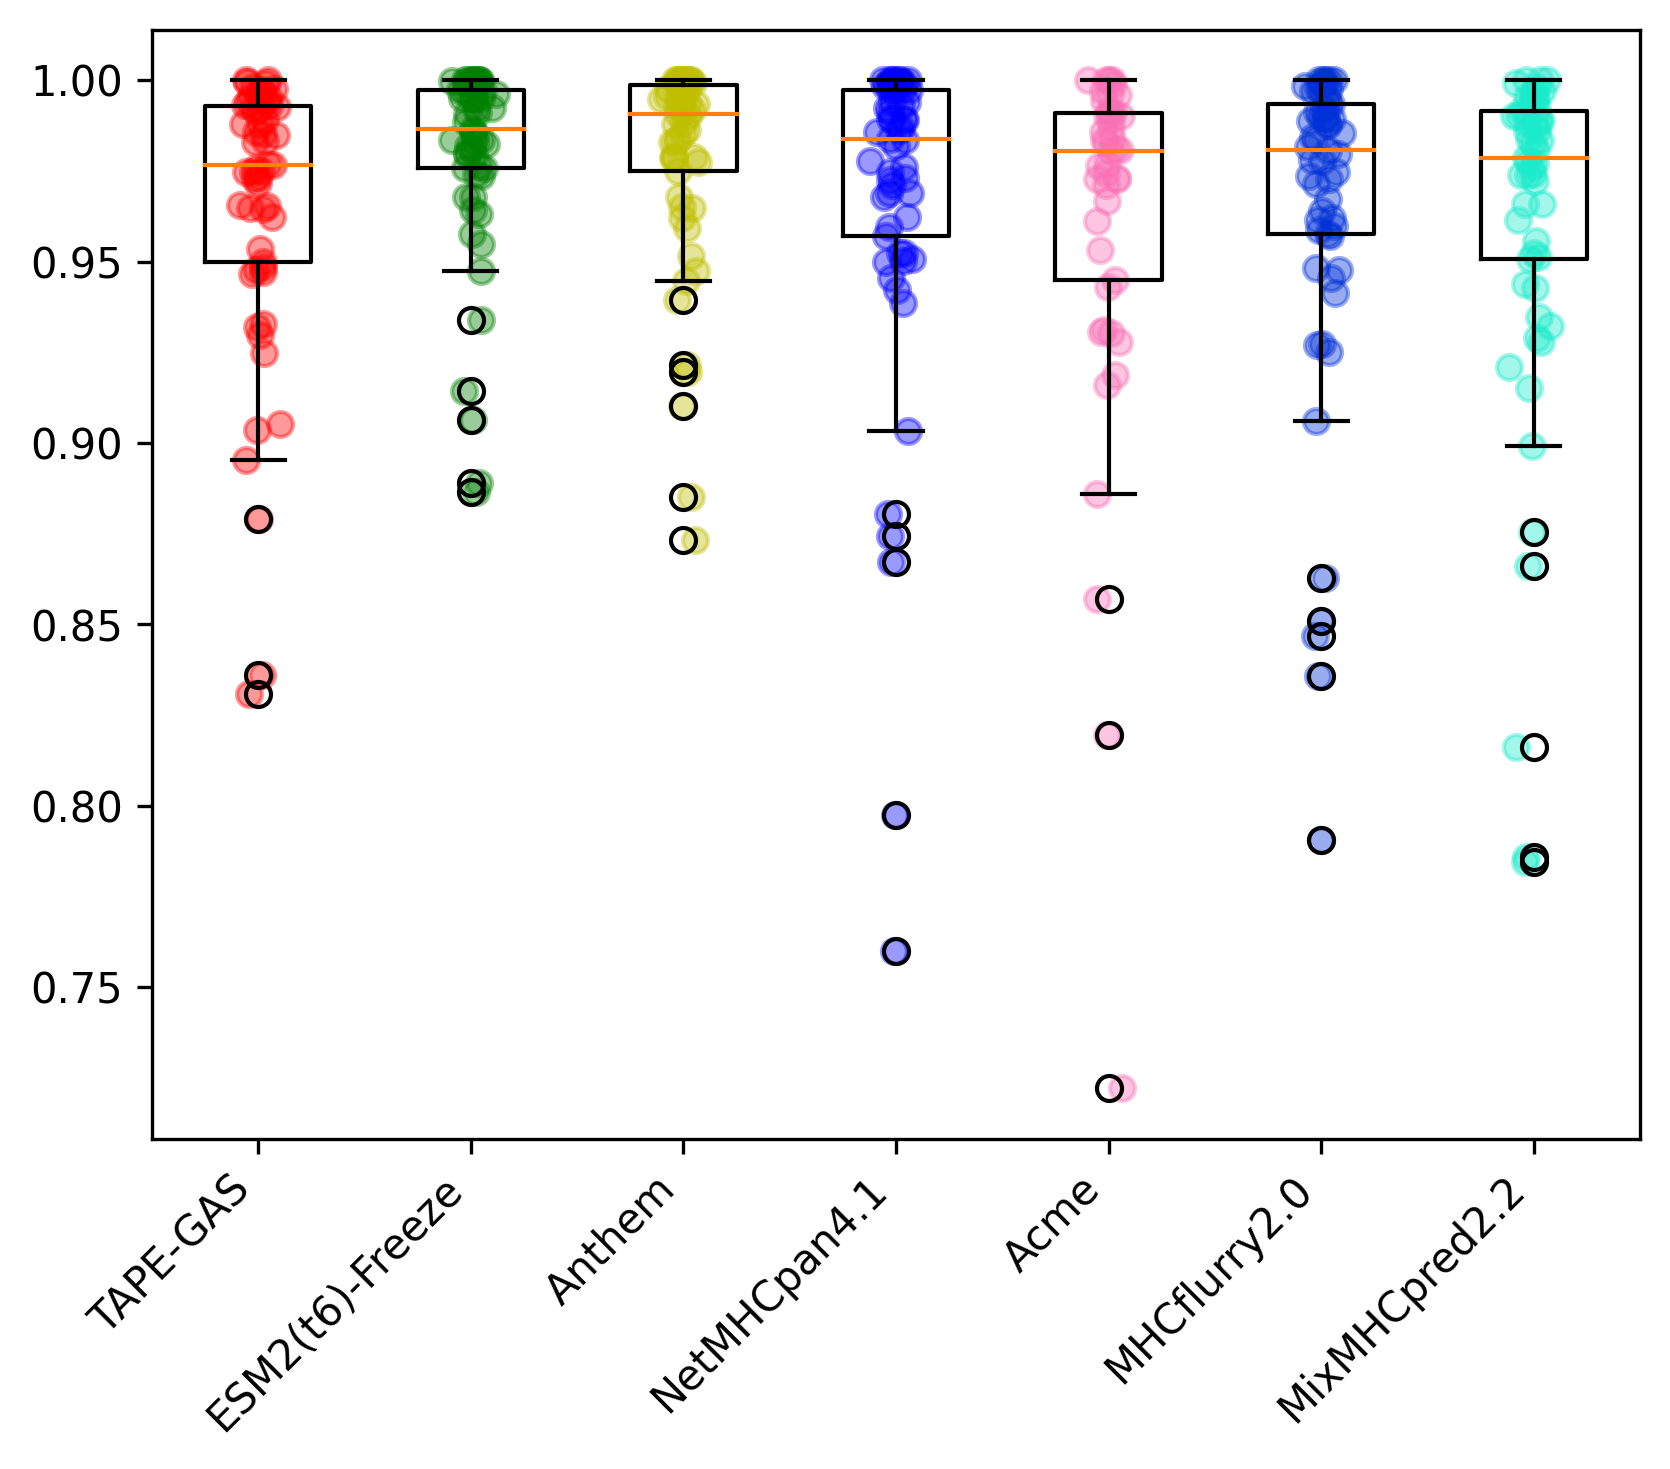
\includegraphics[width=\textwidth]{../img/results/auc_distribution_11-mer}
		\caption{11-mer}
		\label{fig:comparison_11}
	\end{subfigure}
	\hfill
	\begin{subfigure}[b]{0.3\textwidth}
		\centering
		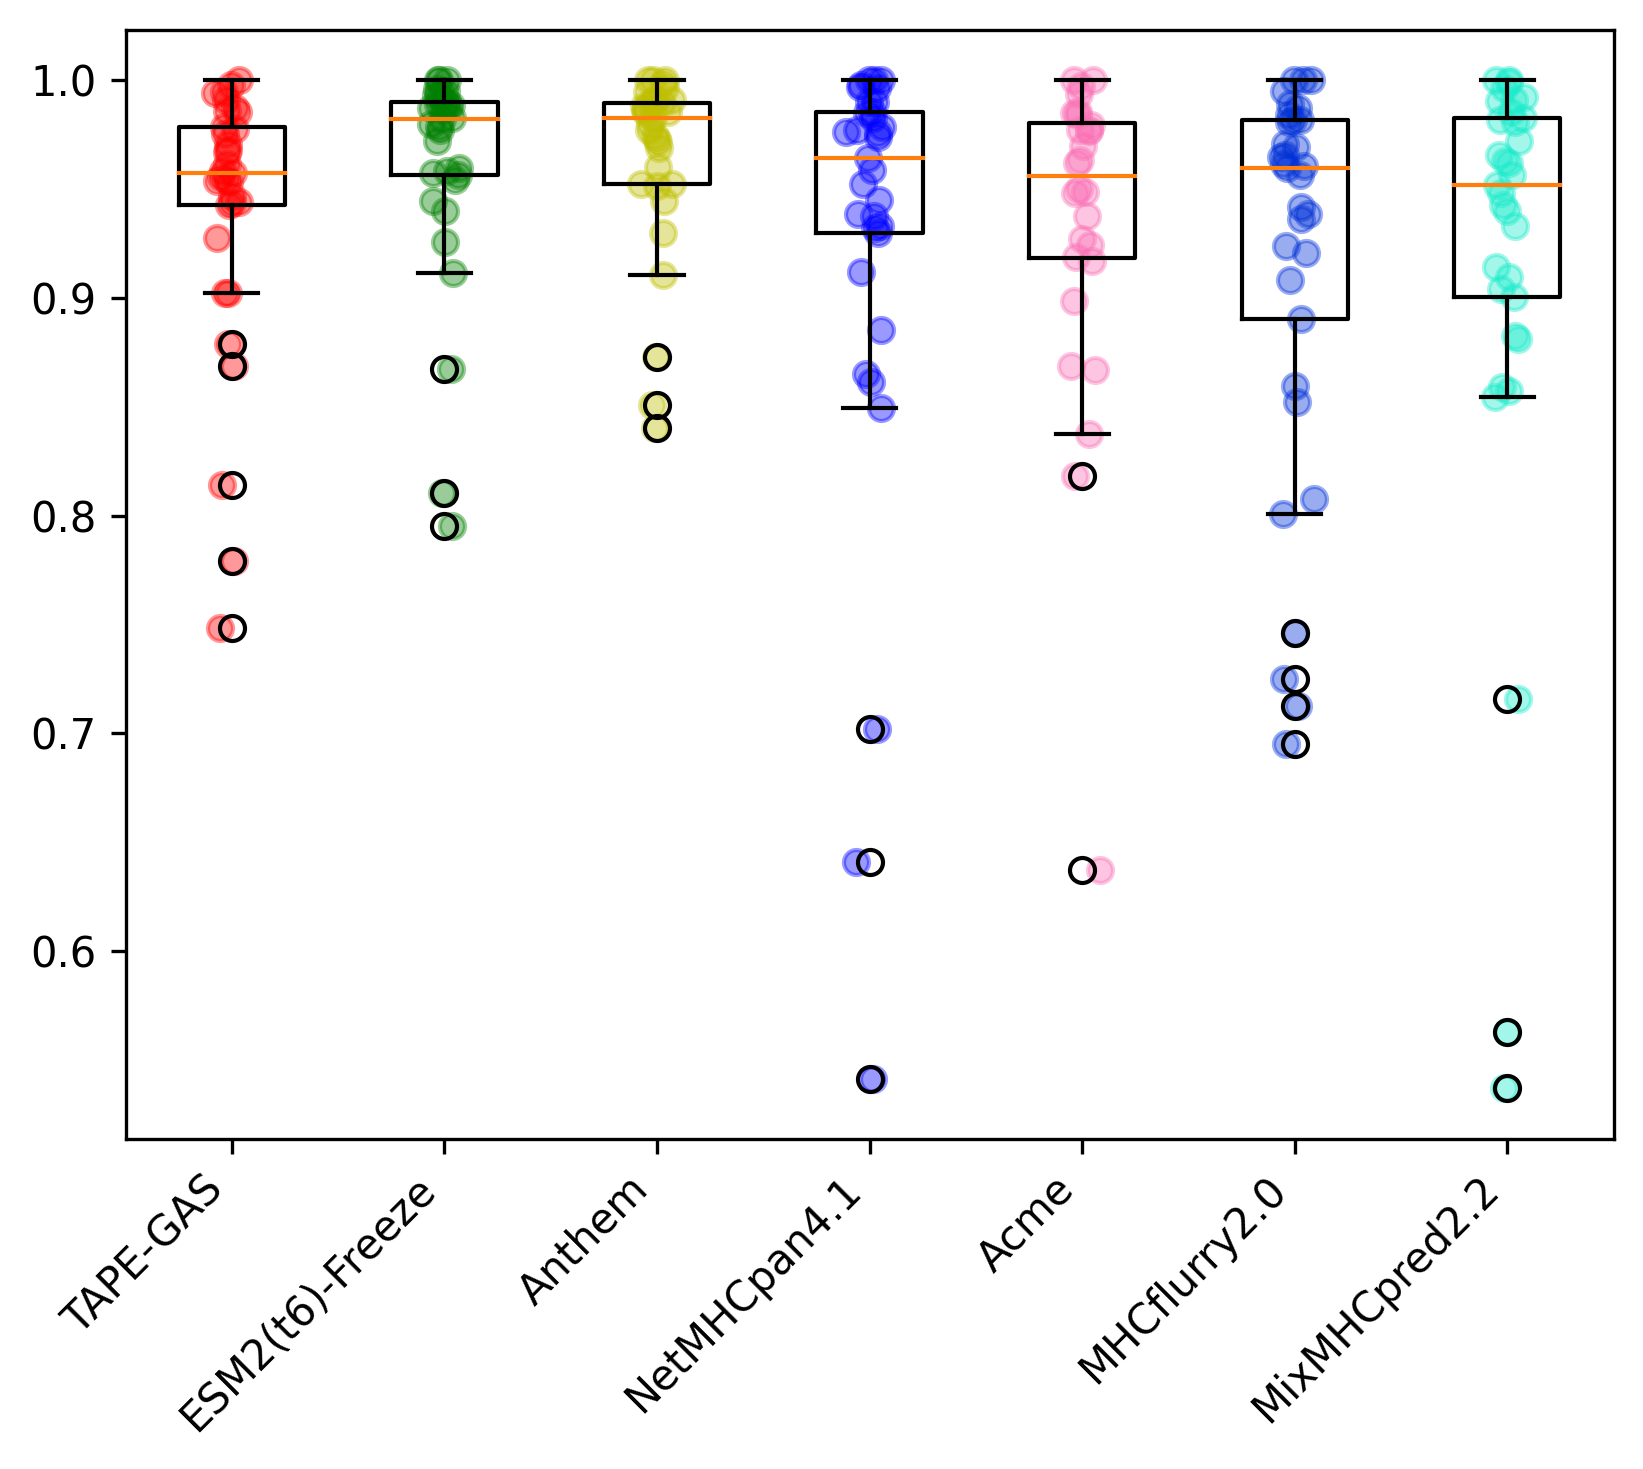
\includegraphics[width=\textwidth]{../img/results/auc_distribution_12-mer}
		\caption{12-mer}
		\label{fig:comparison_12}
	\end{subfigure}
	\hfill
	\begin{subfigure}[b]{0.3\textwidth}
		\centering
		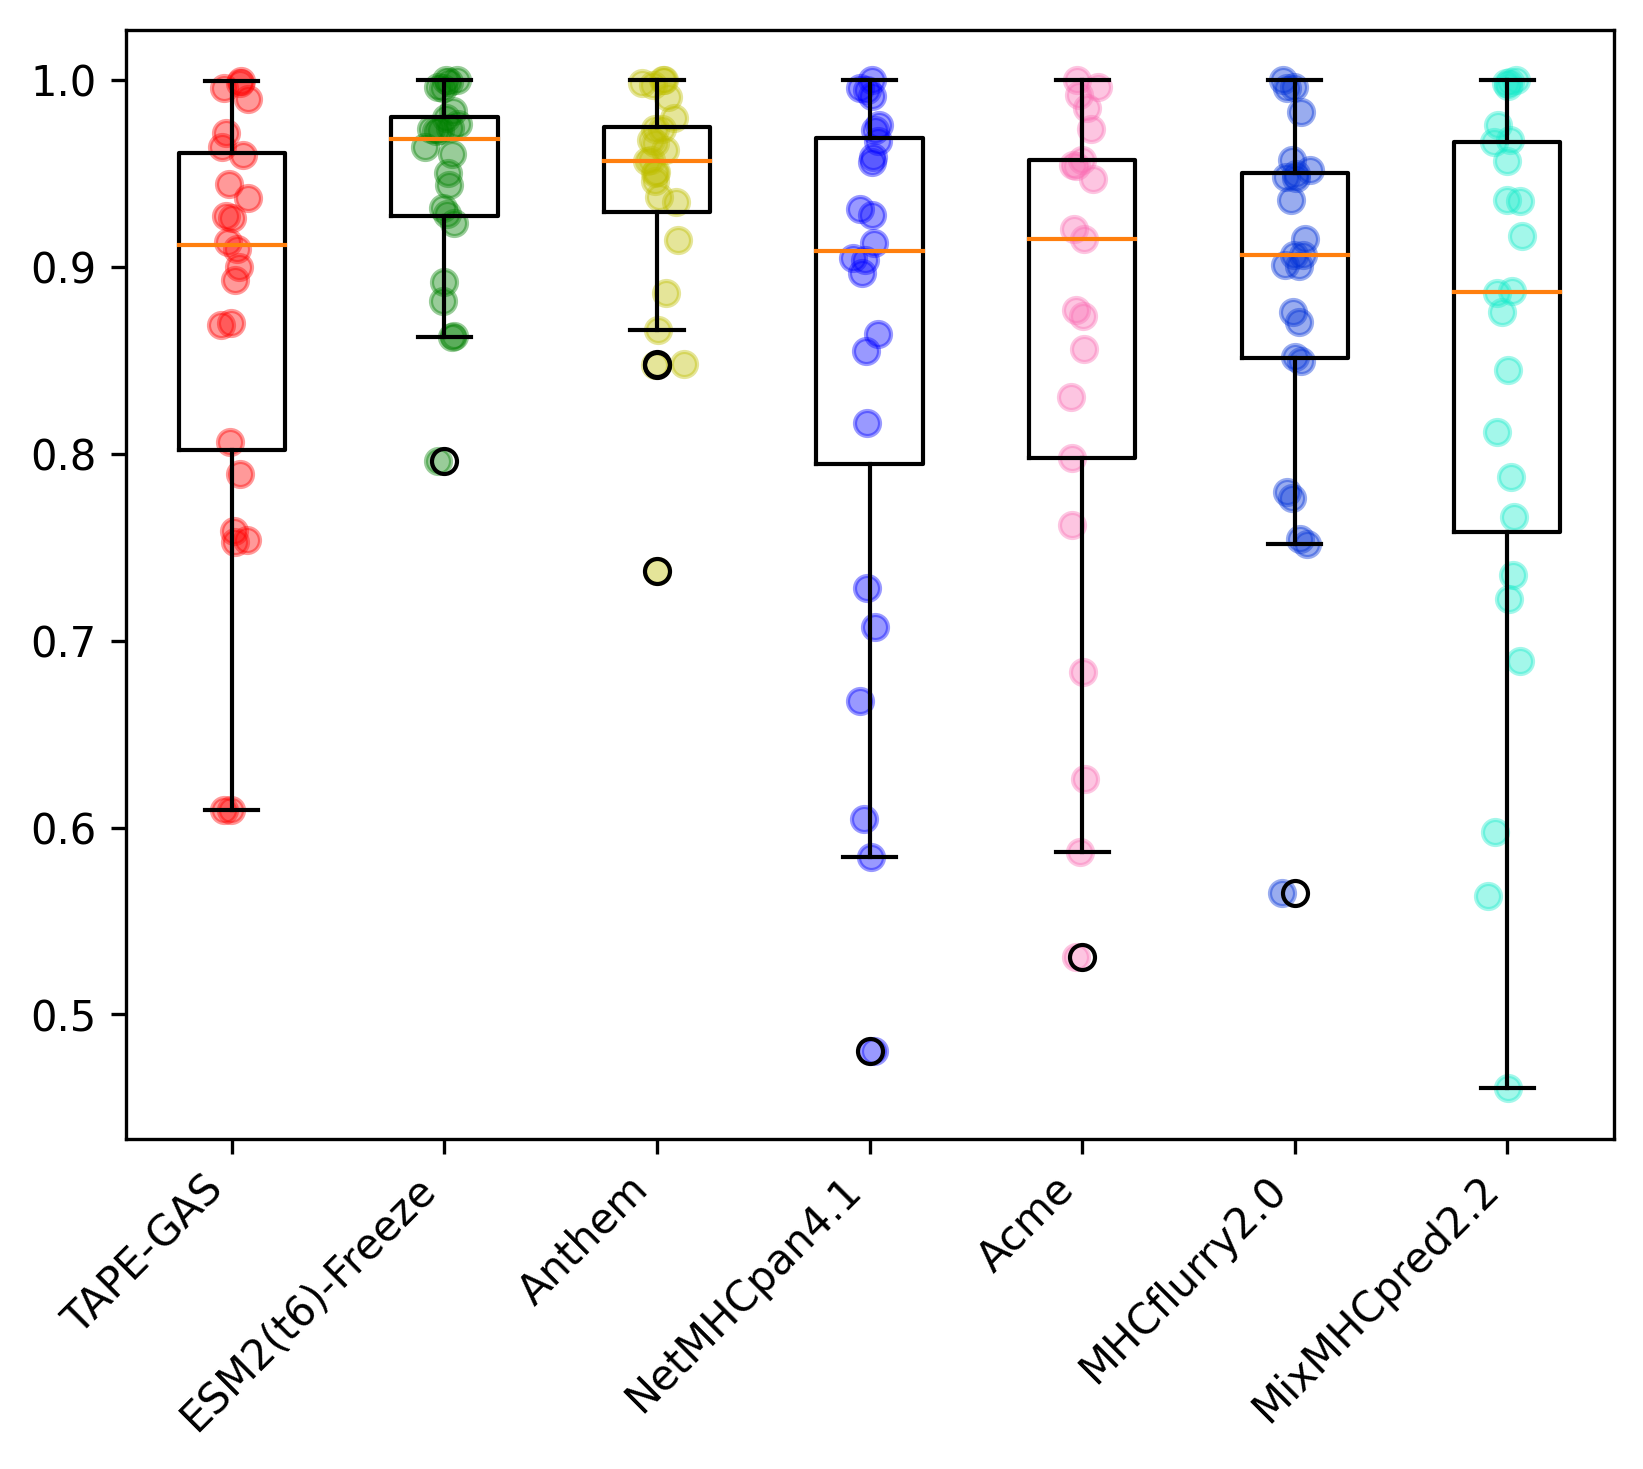
\includegraphics[width=\textwidth]{../img/results/auc_distribution_13-mer}
		\caption{13-mer}
		\label{fig:comparison_13}
	\end{subfigure}
	\hfill
	\begin{subfigure}[b]{0.3\textwidth}
		\centering
		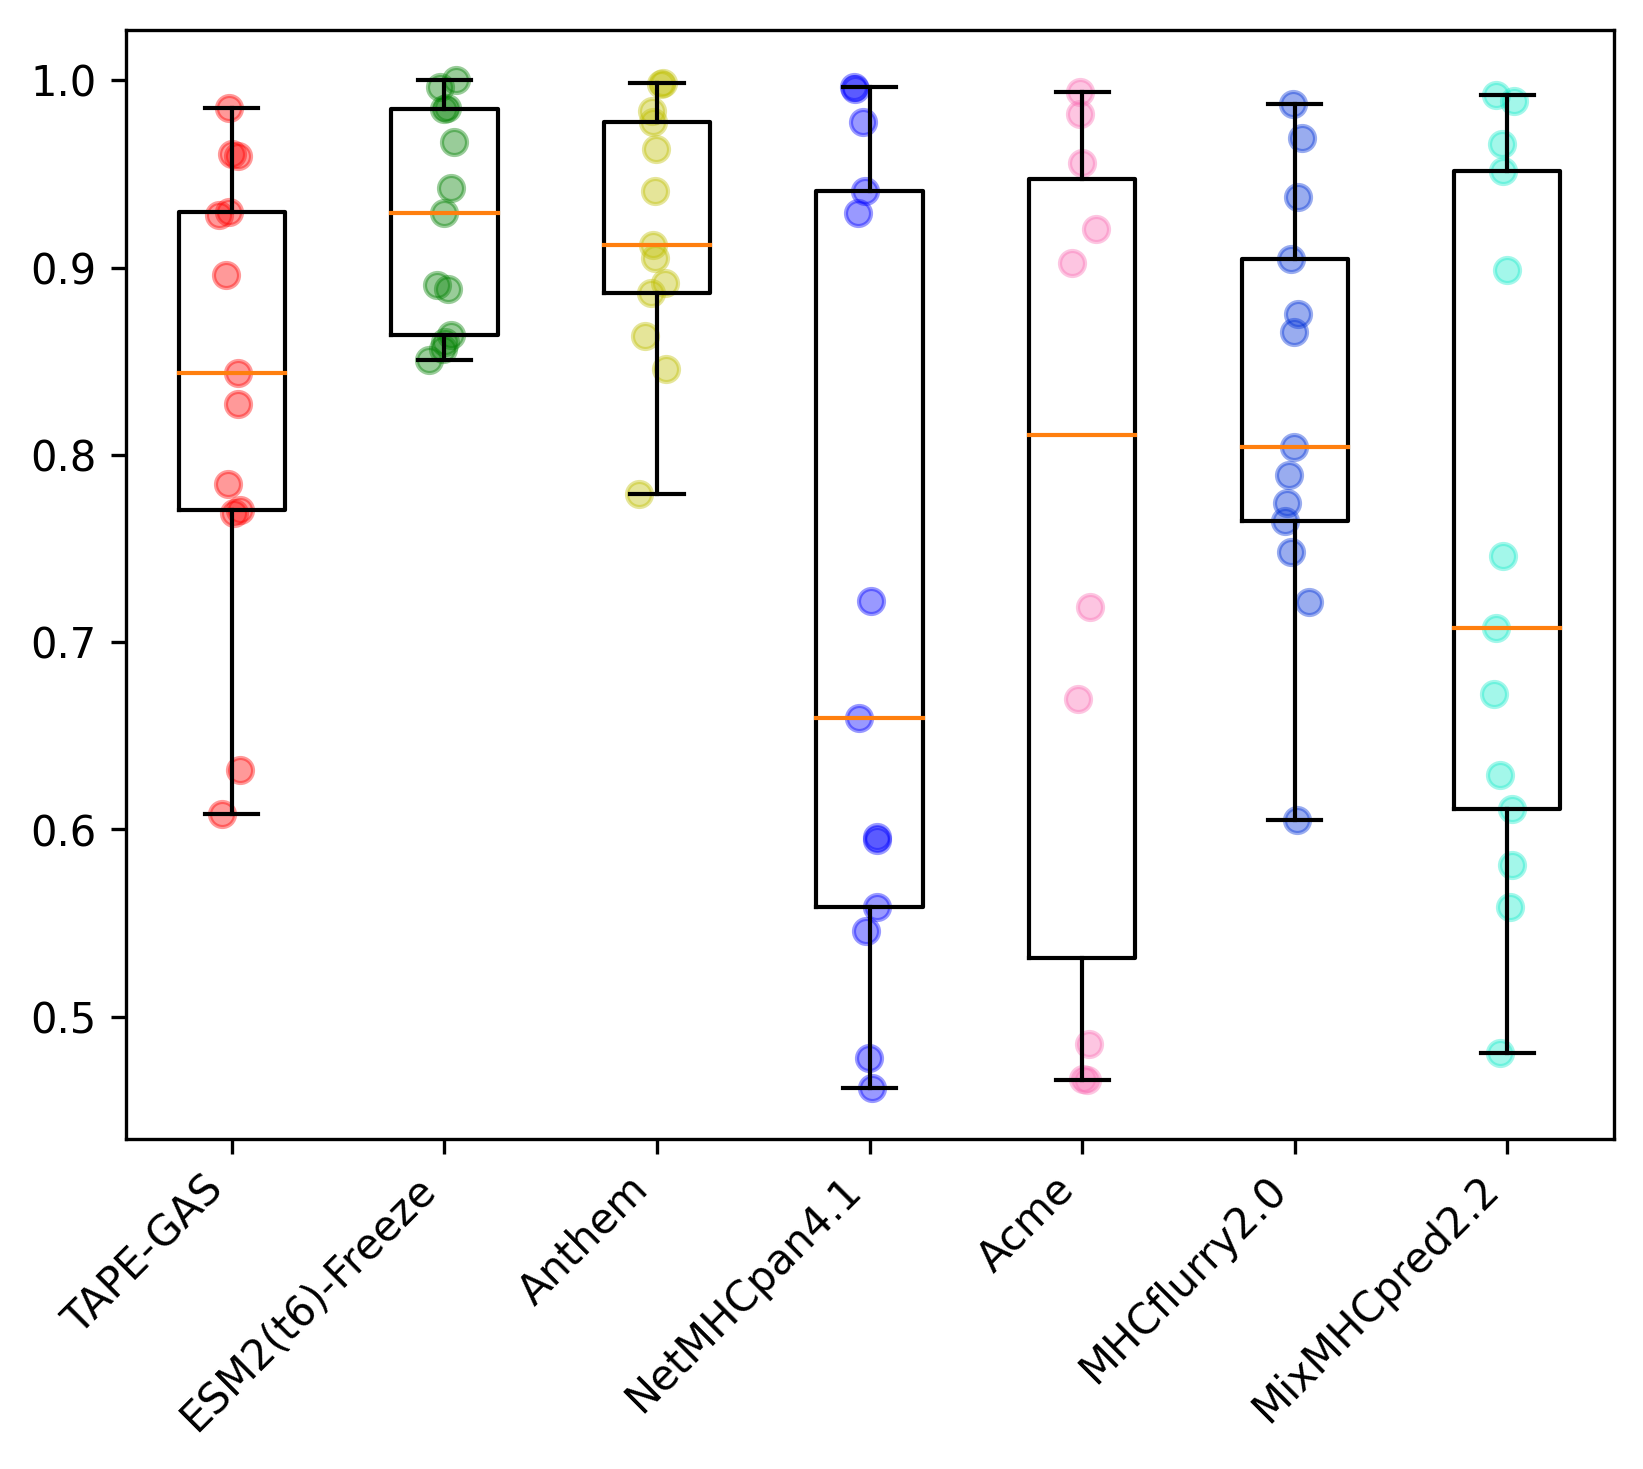
\includegraphics[width=\textwidth]{../img/results/auc_distribution_14-mer}
		\caption{14-mer}
		\label{fig:comparison_14}
	\end{subfigure}
	\caption{The AUC distribution for TAPE-GAS and ESM2(t6)-Freeze, both trained for 30 epochs, along with Anthem, NetMHCpan4.1, ACME, MixMHCpred2.2, and MHCflurry2.0.}
	\label{fig:auc_distribution}
\end{figure*}

\input{5_results}
\section{Discussion}

%\subsection{Fine-tuning ESM2 models}
When specifically considering ESM2 Transformer models, the most favorable results were obtained with the smallest model, ESM2(t6), as indicated in Table \ref{tab:comparison_3_epochs}. However, it's noteworthy that the authors of ESM2 reported in their paper that for various other tasks, larger models like ESM2(t30) and ESM2(t33) outperformed the smaller ones such as ESM2(t6) and ESM2(t12) \cite{lin2023evolutionary}. Additionally, it is well-established that larger models tend to exhibit faster learning but require more extensive training datasets \cite{elnaggar2021prottrans}. In the case of pMHC-I binding prediction, our study employed a dataset comprising 559,019 samples, which we believe is not sufficiently large for ESM2(t33), a model boasting 650 million parameters. In future research endeavors, we plan to assess the performance of larger models using more extensive datasets. Another potential reason for the superior performance of ESM2(t6) could be attributed to the use of Rotary Position Embedding (RoPE) used instead of absolute positional encoding. While RoPE may lead to a slight increase in training cost, it has been observed to enhance the quality of results, particularly for smaller models \cite{lin2023evolutionary}.

%\subsection{Layer Freezing and GAS}


During the training of Transformer models, we explored the implementation of a layer freezing methodology. This approach involves locking the Transformer model while updating only the BiLSTM parameters. As reported in various studies on freezing methodologies in Transformers \cite{merchant2020happens,lee2019would,kovaleva2019revealing}, this method is generally well-suited to accelerate the training process, even though it may lead to a slight sacrifice in performance. Surprisingly, for ESM2 models, this methodology yielded the best results. Moreover, we encountered a recurring issue of vanishing gradients when training large models such as TAPE-normal, ProtBert-normal, ESM2(t30)-normal, and ESM2(t33)-normal. This challenge is a common occurrence when training large language models, as gradients tend to approach zero values after several training steps. To address this, we reduce the learning rate and increased the warmup steps.


%\subsection{TAPE, ProtBert-BFD and ESM2}
Furthermore, a comparison between TAPE, ProtBert-BFD, and ESM2, each of one described in Table \ref{tab:pretrained}. The metrics are presented in Table \ref{tab:comparison_3_epochs}. According to this information, ProtBert-BFD got the worst result despite the fact this model was pre-trained with the largest dataset BFD with 2122M samples; moreover, it has 420M parameters. We believe this result is caused by the noisy information and sequence mistakes in the BFD dataset \cite{elnaggar2021prottrans}. Moreover, large Transformers models need more data for training \cite{elnaggar2021prottrans}, and we fine-tuned this model with 559019 samples.

Additionally, it is notable that TAPE achieved the best results, with ESM2(t6) following closely (as shown in Table \ref{tab:comparison_3_epochs}). TAPE models were pre-trained using the Pfam dataset, which is the smallest dataset in this comparison, containing approximately 30 million samples. It's important to mention that the Pfam dataset is derived from UniProtKB and selectively includes sequences belonging to Reference Proteomes rather than encompassing the entire UniProtKB database \cite{finn2016pfam}. Consequently, Pfam covers half of the protein sequences compared to other datasets based on UniProtKB, but its samples are of higher quality. Therefore, it is plausible to assume that TAPE encapsulates a more comprehensive and refined representation of protein information compared to other pre-trained models. Moreover, ESM2(t6) achieved results that closely rival TAPE's performance, as demonstrated in Table \ref{tab:comparison}. Notably, ESM2(t6) comprises only 8 million parameters, compared to 92 million parameters of TAPE. Furthermore, both models were trained on samples from UniProtKB, although TAPE used a subset of this dataset. Moreover, ESM2(t6) outperformed TAPE for longer peptides, ranging from 11 to 14 mers, as depicted in Fig. \ref{fig:auc_distribution}. These findings strongly position ESM2(t6) as a prime candidate for future analyses due to its remarkable performance and cost-effectiveness.


\section{Conclusions}

In our comparative analysis of the six Transformer models TAPE, ProtBert-BFD, ESM2(t6), ESM2(t12), ESM2(t30), and ESM2(t33) with the incorporation of GAS and the layer freezing technique, we observed that ESM2(t6)-Freeze, and TAPE-GAS achieved the most favorable outcomes. Additionally, we found that the layer freezing methodology accelerated the training process and produced the most favorable results for ESM2 models. In contrast, using GAS led to the best results for TAPE and ProtBert.

Moreover, after training ESM2(t6)-Freeze and TAPE-GAS for thirty epochs, the models surpassed state-of-the-art methods, including NetMHCpan4.1, MHCflurry2.0, Anthem, ACME, and MixMHCpred2.2, in terms of various performance metrics like AUC, accuracy, recall, f1-score, and MCC. This demonstrates the advantages of fine-tuning large Transformer models for predicting peptide-MHC binding, underscoring their potential to enhance this critical task.

Additionally, the vanishing gradient problem is a common problem when training large BERT models. So, in order to avoid this problem, we noticed that larger models need very small learning rates at the beginning of training. Furthermore, in order to maintain stability, it is very useful to use a scheduler to increase and decrease the learning rate during training. Thus, after experiments, we managed to use a learning rate of $2e-6$ and 200k step for warnup. Additionally, we used the ADAM optimizer with bias correction.

\section{Future works}
In this work, we evaluated TAPE, ProtBert-BFD, ESM2(t6), ESM2(t12), ESM2(t30), and ESM2(t33), each one with 92, 420, 8, 35, 150, and 650 million parameters respectively. However, we have other alternatives like ProtT5-XL and ProtT5-XXL, ESM2(t36), and ESM2(t48), each one with 3, 11, 3, and 15 billion parameters, respectively. We didn't evaluate these models because of the small size of the dataset and the training cost. Nevertheless, we planned to evaluate these huge Transformer models with a large dataset comprising samples from Anthem dataset \cite{mei2021anthem}, MixMHXpred2.2  \cite{gfeller2023improved}, and the most recent benchmarking of pMHC binding prediction tools \cite{wang2023comprehensive}.

Moreover, given the considerable training cost associated with training large Transformer models, we plan to investigate the potential advantages of utilizing DistilBERT \cite{sanh2019distilbert} and LoRA \cite{hu2021lora} for training and future prediction tasks.

Furthermore, we fine-tuned each Transformer model, adding a BiLSTM block at the end, based on the work of HLAB \cite{zhang2022hlab}. Looking ahead, we plan to assess the effectiveness of a Star-Transformer block, similar to the methodology employed in SMHCpan \cite{ye2023stmhcpan}. Furthermore, considering the promising results demonstrated in ESM-GAT \cite{hashemi2023improved}, we believe that the inclusion of a Graph Attention Network (GAT) could significantly enhance our model's performance in future research. Finally, we would like to evaluate the methodology used by TransPHLA \cite{chu2022transformer}, due to its demonstrated effectiveness in handling peptides of different lengths.
%\newpage
\section*{Appendix (if necessary)} 
Please, indicate in your e-mail message the name and e-mail address of the author who will be the contact for the submitted paper. 


%\section*{Acknowledgment}
%This document has been adapted from the CLEI'2004 Conference Proceedings Format specifications, and from previous versions of the CLEIej instructions for authors (2009 version by Mauricio Solar, 2011 version by H�ctor Cancela).  
 
%\bibliographystyle{./IEEEtran}
\bibliography{../bibliography_thesis}

\end{document}

